\documentclass[conference]{IEEEtran}
\IEEEoverridecommandlockouts

\usepackage{cite}
\usepackage{amsmath,amssymb,amsfonts}
\usepackage{graphicx}
\usepackage{textcomp}
\usepackage{xcolor}
\usepackage{hyperref}
\usepackage{booktabs}
\usepackage{multirow}
\usepackage{array}
\usepackage{float}
\usepackage{subcaption}
\usepackage{siunitx}
\usepackage{listings}

\hypersetup{
  colorlinks=true,
  linkcolor=blue,
  citecolor=blue,
  urlcolor=blue
}

\title{Natural Language Processing Assignment 2:\\\
From-Scratch Email Classification and\\
Feature-Driven Phishing URL Detection}

\author{\IEEEauthorblockN{Mohammad Mahdi Salmani Zarchi}
\IEEEauthorblockA{\textit{Department of Computer Engineering} \\
\textit{University of Tehran}\\
Student ID: 810100XXX \\
Email: m.salmani@ut.ac.ir}
}

\begin{document}

\maketitle

\begin{abstract}
This report presents a complete implementation and analysis of two binary classification tasks in Natural Language Processing and security-oriented text analytics. In Question 1, Logistic Regression and Multinomial Naive Bayes are implemented from scratch to classify emails as spam or ham, supported by custom metric functions and Bag-of-Words preprocessing. In Question 2, the same model family is evaluated on phishing URL detection using four feature configurations: structural, statistical/content, creative handcrafted, and combined features. Beyond model training, this work establishes a reproducible pipeline with deterministic data loading, robust label normalization, and automatic figure export for report integration. Experimental results show that from-scratch Logistic Regression outperforms from-scratch Naive Bayes on the email task, while in URL detection the combined feature space substantially improves both methods and highlights precision-recall tradeoffs between discriminative and probabilistic models. The final artifact includes a fully executable notebook and a complete IEEE-format technical report.
\end{abstract}

\begin{IEEEkeywords}
Spam classification, phishing URL detection, Logistic Regression, Naive Bayes, Bag-of-Words, feature engineering, reproducibility
\end{IEEEkeywords}

\section{Introduction}

Email spam filtering and phishing URL detection are two foundational binary classification tasks with direct operational impact in real-world communication systems. Although both tasks are commonly solved with off-the-shelf machine learning pipelines, educational assignments that require step-by-step implementation reveal practical failure modes that are often hidden in automated toolchains. This report documents a full completion of Assignment 2 with an emphasis on correctness, reproducibility, and technical analysis.

The work is divided into two questions. Question 1 focuses on text classification with strict implementation constraints: Logistic Regression and Multinomial Naive Bayes are built from scratch, and evaluation metrics are manually implemented. Question 2 shifts from free text to URL strings and allows library usage; the main challenge becomes feature engineering and model behavior interpretation under different feature families.

A key objective of this submission is not only to obtain competitive accuracy, but also to produce a stable experiment artifact that can be rerun without hidden assumptions. During development, several engineering issues were resolved: path-dependent dataset loading, missing dependency handling, non-deterministic split failures on fallback data, and missing report figure exports. The final notebook now loads all datasets from fixed CA2 paths, performs robust label normalization, exports deterministic plots for reporting, and executes fully in a clean run.

\subsection{Datasets and Task Definitions}

\textbf{Question 1 data:}
\begin{itemize}
    \item \texttt{emails\_1.csv}: a compact labeled set with raw text and labels \texttt{spam}/\texttt{ham}.
    \item \texttt{emails\_2.csv}: a larger Bag-of-Words matrix with 5172 emails, 3000 vocabulary features, and a \texttt{Prediction} label column.
\end{itemize}

\textbf{Question 2 data:}
\begin{itemize}
    \item \texttt{urls.csv}: 11,430 URL samples with balanced labels \texttt{phishing}/\texttt{legitimate}.
\end{itemize}

Both problems are binary classification tasks. We report Accuracy, Precision, Recall, and F1-score throughout, and include confusion matrices and ranking-curve visualizations for interpretability.

\subsection{Contributions of This Report}

This report provides four concrete contributions:
\begin{enumerate}
    \item A complete from-scratch implementation of Question 1 models and metrics with reproducible preprocessing.
    \item A structured feature-engineering study for phishing URL detection across multiple feature families.
    \item A deterministic figure generation pipeline producing report-ready plots directly from notebook execution.
    \item A consolidated IEEE-format technical narrative linking implementation choices to measured behavior.
\end{enumerate}

The remainder of this report follows the assignment flow while adding engineering-level analysis and reproducibility details.

\section{Question 1: Methods and Implementation}

\subsection{Preprocessing and Bag-of-Words}

The first stage uses \texttt{emails\_1.csv} to demonstrate preprocessing and sparse lexical representation. Labels are normalized by mapping \texttt{spam} $\rightarrow 1$ and \texttt{ham} $\rightarrow 0$. Text is cleaned by removing non-alphabetic symbols and converting to lowercase. A CountVectorizer with \texttt{max\_features=15} is then used to construct a compact Bag-of-Words (BoW) representation.

This stage serves two roles: (i) verifying the preprocessing logic required by the assignment, and (ii) generating interpretable lexical statistics for report visualization.

\subsection{Training Data for Model Learning}

For model training, we use \texttt{emails\_2.csv}, which already contains BoW-style numeric features at scale. The pipeline performs the following transformations:
\begin{enumerate}
    \item Read CSV from fixed project path.
    \item Use \texttt{Prediction} (or \texttt{status} if present) as the binary target.
    \item Drop non-feature identifiers such as \texttt{Email No.}.
    \item Coerce all feature columns to numeric and fill missing values with 0.
\end{enumerate}

The final matrix has 5172 samples with a class distribution of 3672 ham and 1500 spam, preserving moderate imbalance representative of operational email streams.

\subsection{Train/Test Split and Reproducibility}

A fixed random seed is used with an 80/20 train-test split. Stratification is applied when class counts permit safe stratified partitioning. A helper guard disables stratification only in edge cases where a fallback mini-dataset would otherwise make stratified splitting invalid. This avoids silent runtime crashes while preserving expected behavior on the real dataset.

\subsection{Manual Evaluation Metrics}

The assignment requires manual implementations of binary classification metrics. Let TP, TN, FP, and FN denote confusion matrix counts. The metric definitions are:
\begin{align}
\text{Accuracy} &= \frac{TP + TN}{TP + TN + FP + FN} \\
\text{Precision} &= \frac{TP}{TP + FP} \\
\text{Recall} &= \frac{TP}{TP + FN} \\
F_1 &= \frac{2 \cdot \text{Precision} \cdot \text{Recall}}{\text{Precision} + \text{Recall}}
\end{align}

Zero-division safeguards are included for edge conditions.

\subsection{From-Scratch Logistic Regression}

Logistic Regression is implemented with gradient descent on binary cross-entropy loss:
\begin{align}
\hat{y} &= \sigma(w^Tx + b), \quad \sigma(z)=\frac{1}{1+e^{-z}} \\
\mathcal{L} &= -\frac{1}{N}\sum_{i=1}^{N}\left[y_i\log(\hat{y}_i)+(1-y_i)\log(1-\hat{y}_i)\right]
\end{align}

The implementation includes:
\begin{itemize}
    \item Feature normalization using training-set mean and standard deviation.
    \item Numerically stable sigmoid via clipping.
    \item Fixed learning rate and iteration count.
\end{itemize}

This model is discriminative and can capture correlated feature effects, which is often beneficial in sparse lexical spaces \cite{hastie2009elements,manning2008introduction}.

\subsection{From-Scratch Multinomial Naive Bayes}

Multinomial Naive Bayes is implemented with Laplace smoothing. For class $c$ and feature $j$:
\begin{align}
P(x_j|c) = \frac{N_{jc}+\alpha}{\sum_k N_{kc}+\alpha d}
\end{align}
where $d$ is feature dimension and $\alpha=1.0$. Training uses log probabilities to avoid underflow. Prediction computes:
\begin{align}
\log P(c|x) \propto \log P(c) + \sum_j x_j \log P(x_j|c)
\end{align}

Despite its conditional independence assumption, Multinomial NB remains a strong lexical baseline \cite{mccallum1998comparison}.

\subsection{Reporting Figures for Q1}

To support direct report integration, the notebook exports Q1 figures automatically:
\begin{itemize}
    \item Confusion matrix comparison.
    \item ROC and Precision-Recall curves for Logistic Regression.
    \item Top BoW words per class from \texttt{emails\_1.csv}.
    \item Metric bar chart comparing Logistic Regression vs Naive Bayes.
\end{itemize}

These files are saved under \texttt{answer/report/figures/} with deterministic names.

\section{Question 1: Experimental Results and Analysis}

\subsection{Quantitative Performance}

Table~\ref{tab:q1-main} reports test-set performance for the two from-scratch models on \texttt{emails\_2.csv}.

\begin{table}[H]
\centering
\caption{Question 1 test metrics on \texttt{emails\_2.csv}}
\label{tab:q1-main}
\begin{tabular}{lcc}
\toprule
Metric & Logistic Regression & Naive Bayes \\
\midrule
Accuracy  & 0.9633 & 0.9420 \\
Precision & 0.9199 & 0.8681 \\
Recall    & 0.9567 & 0.9433 \\
F1-score  & 0.9379 & 0.9042 \\
\bottomrule
\end{tabular}
\end{table}

Logistic Regression outperforms Naive Bayes on every metric. The largest practical gain appears in precision and F1-score, suggesting fewer false positives while preserving strong detection of spam emails.

\subsection{Confusion and Ranking Behavior}

\begin{figure}[H]
\centering
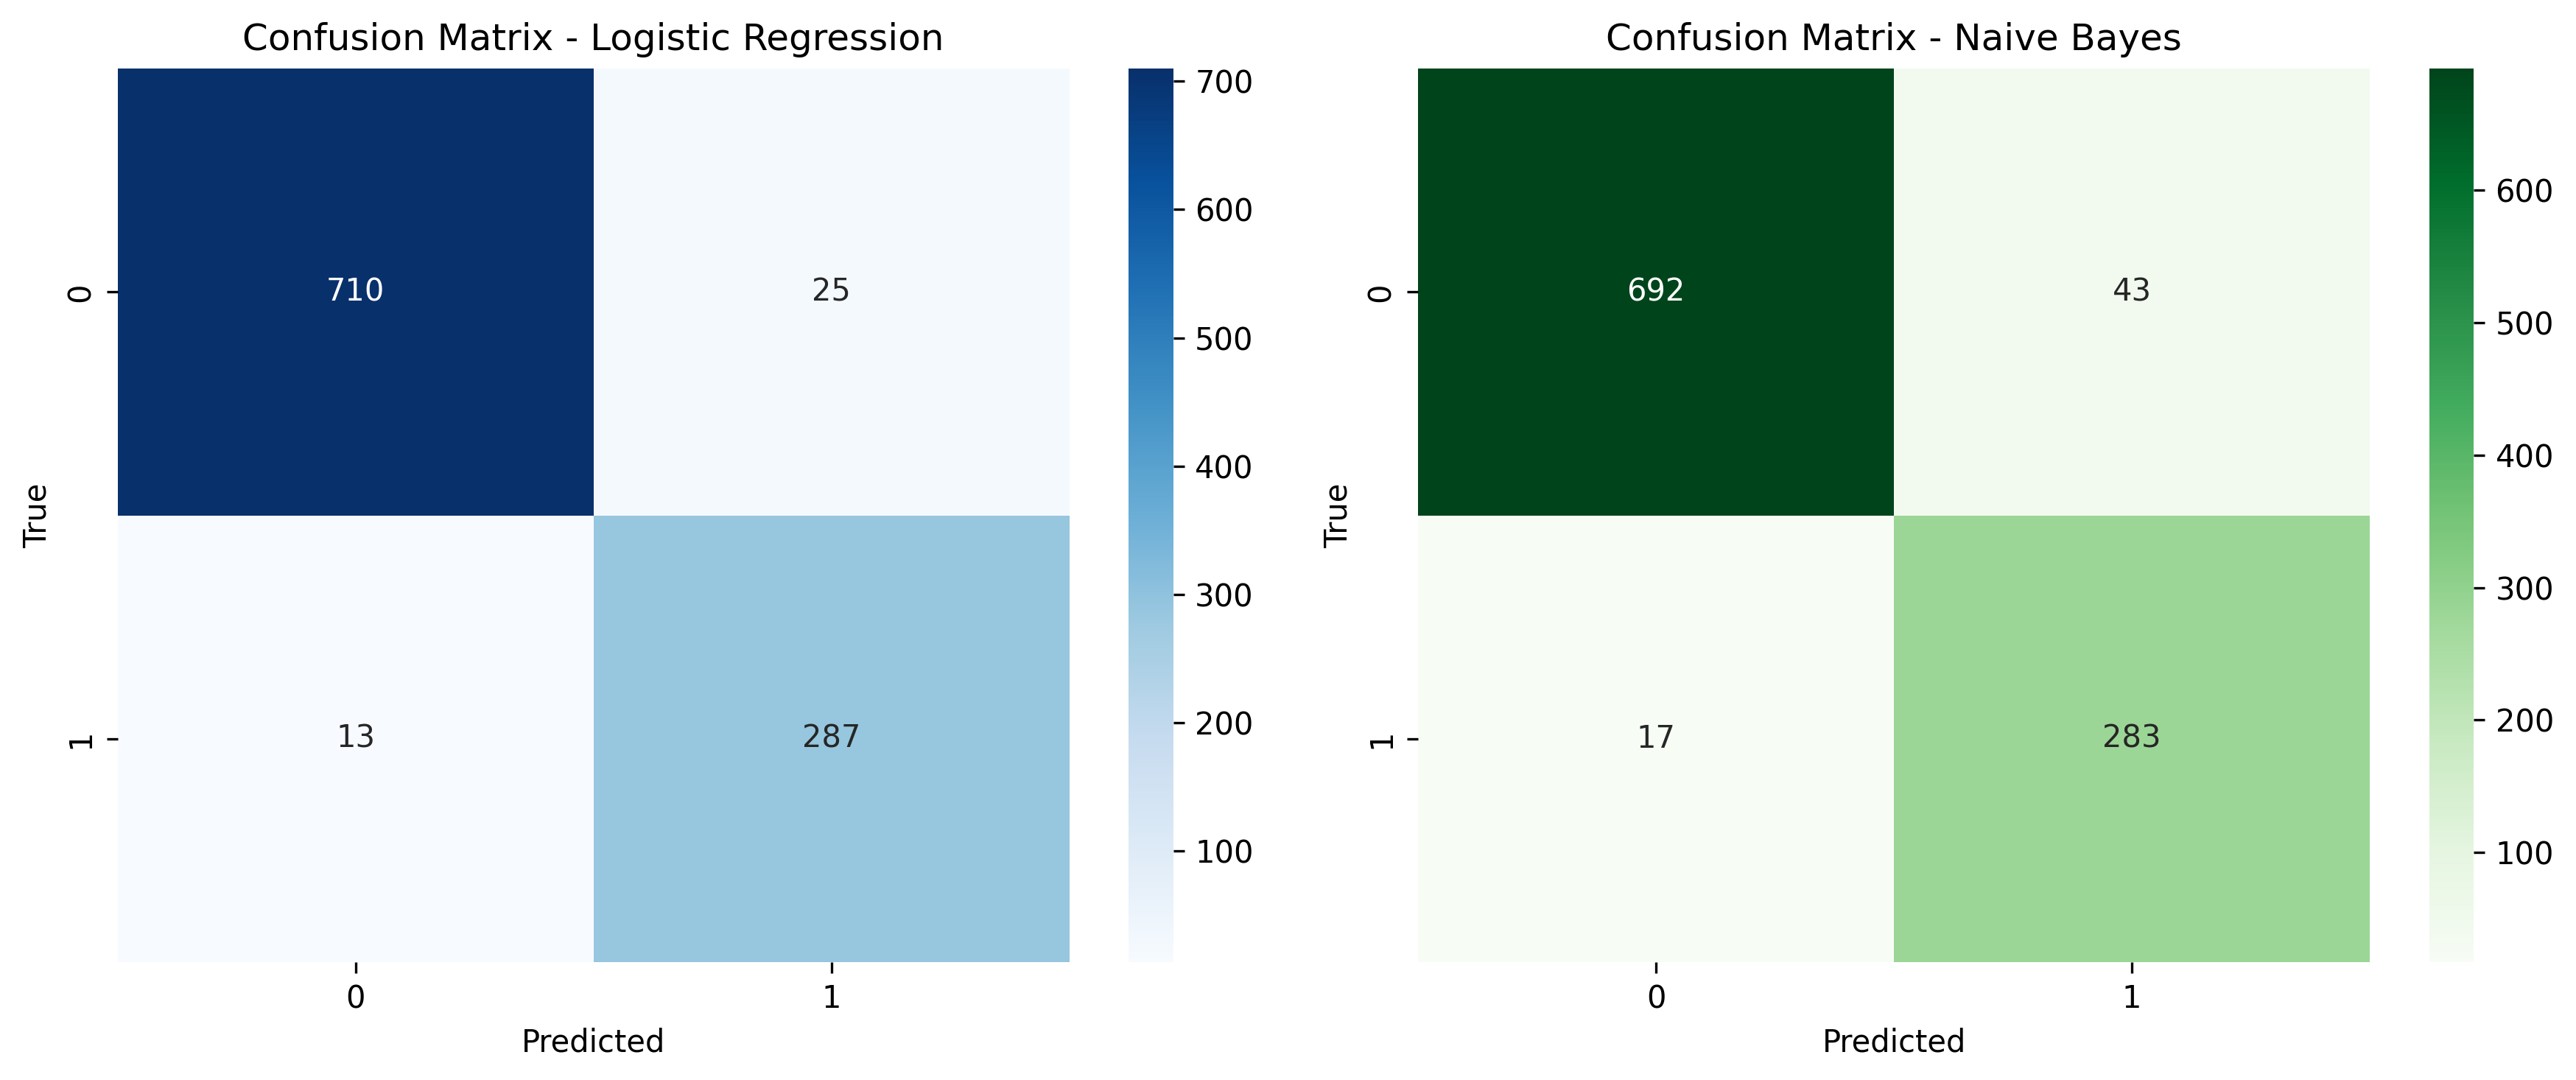
\includegraphics[width=0.48\textwidth]{figures/q1_confusion_matrices.png}
\caption{Confusion matrix comparison for Q1 models.}
\label{fig:q1-cm}
\end{figure}

Figure~\ref{fig:q1-cm} confirms the quantitative result: Logistic Regression provides a cleaner separation between positive and negative classes.

\begin{figure}[H]
\centering
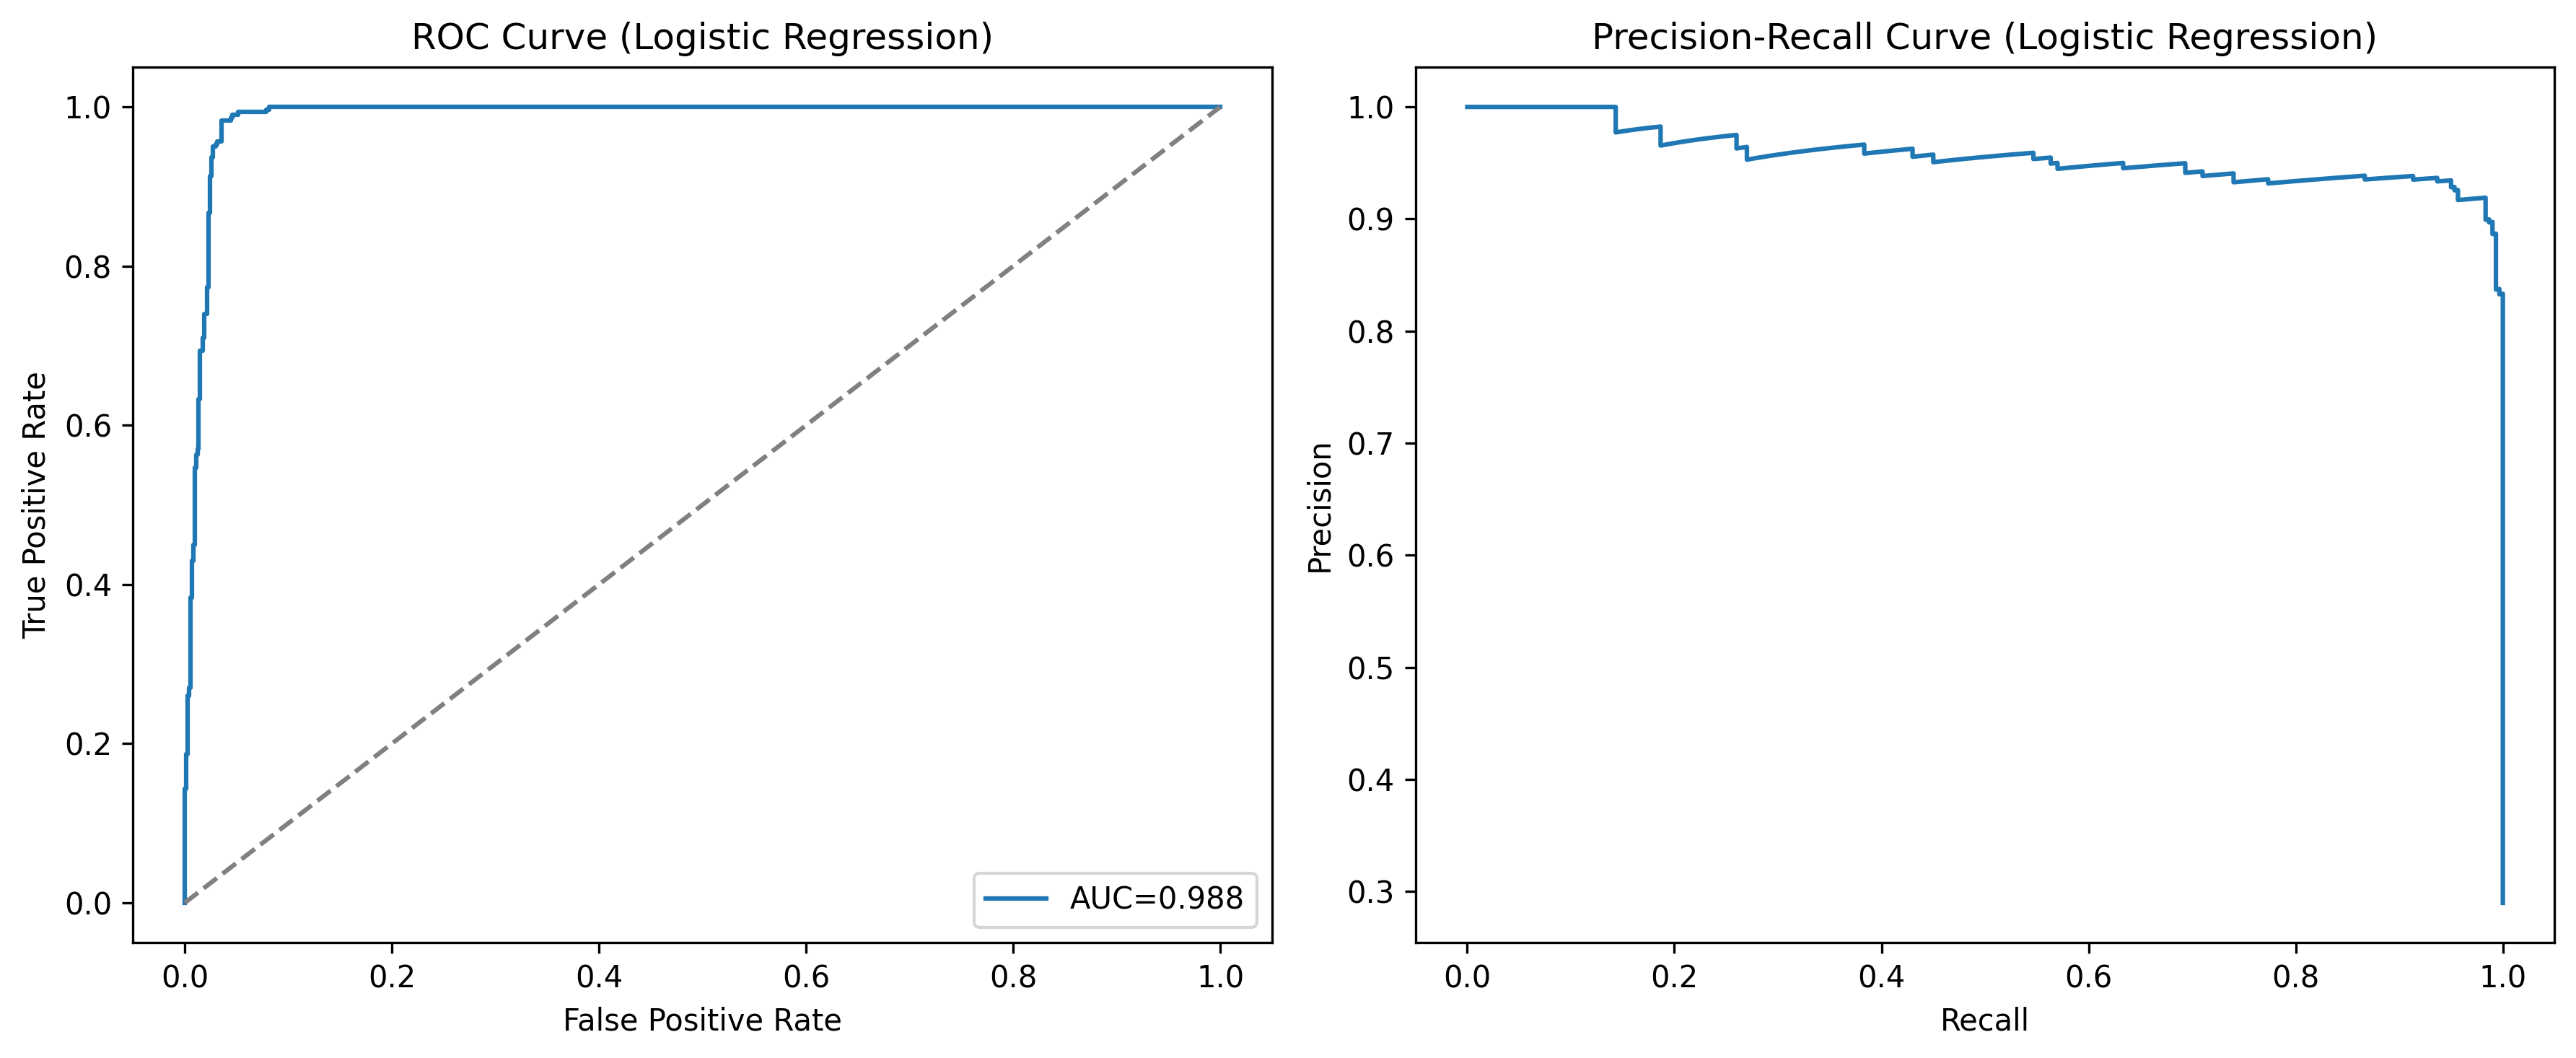
\includegraphics[width=0.48\textwidth]{figures/q1_roc_pr_curves_lr.png}
\caption{ROC and Precision-Recall curves for from-scratch Logistic Regression.}
\label{fig:q1-roc-pr}
\end{figure}

The ROC/PR visualization in Figure~\ref{fig:q1-roc-pr} demonstrates robust ranking quality and threshold flexibility, important for downstream tuning under varying business costs.

\subsection{Lexical Interpretation}

\begin{figure}[H]
\centering
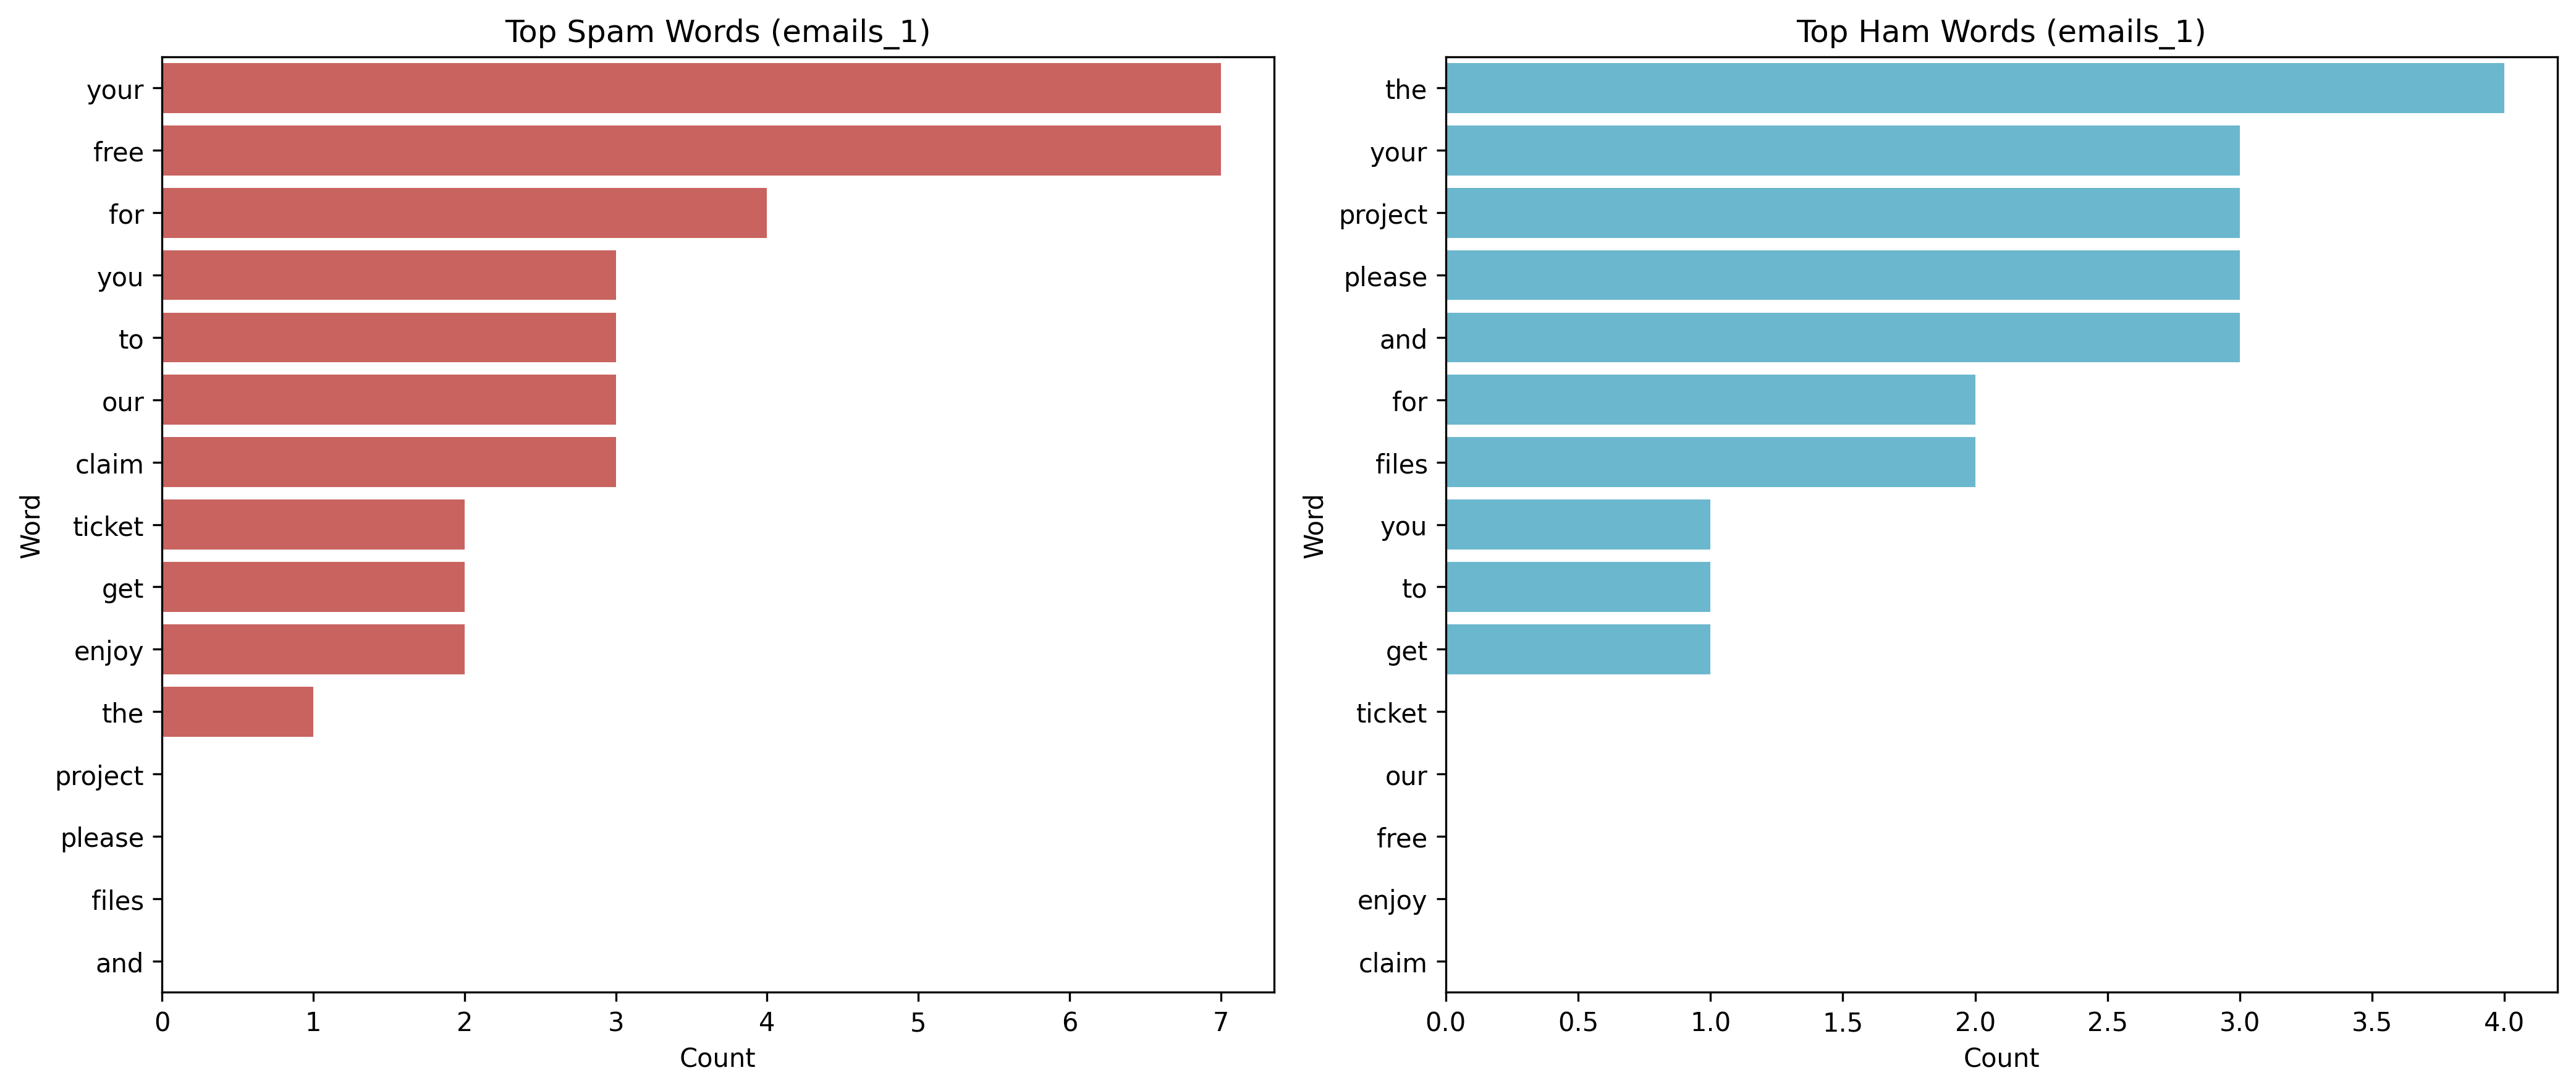
\includegraphics[width=0.48\textwidth]{figures/q1_top_words_spam_ham.png}
\caption{Top class-specific terms from the BoW projection of \texttt{emails\_1.csv}.}
\label{fig:q1-words}
\end{figure}

Figure~\ref{fig:q1-words} highlights class-discriminative lexical signals. Although this mini-dataset is not used for main model training, it helps validate preprocessing assumptions and demonstrates why token-frequency models remain competitive for spam filtering.

\begin{figure}[H]
\centering
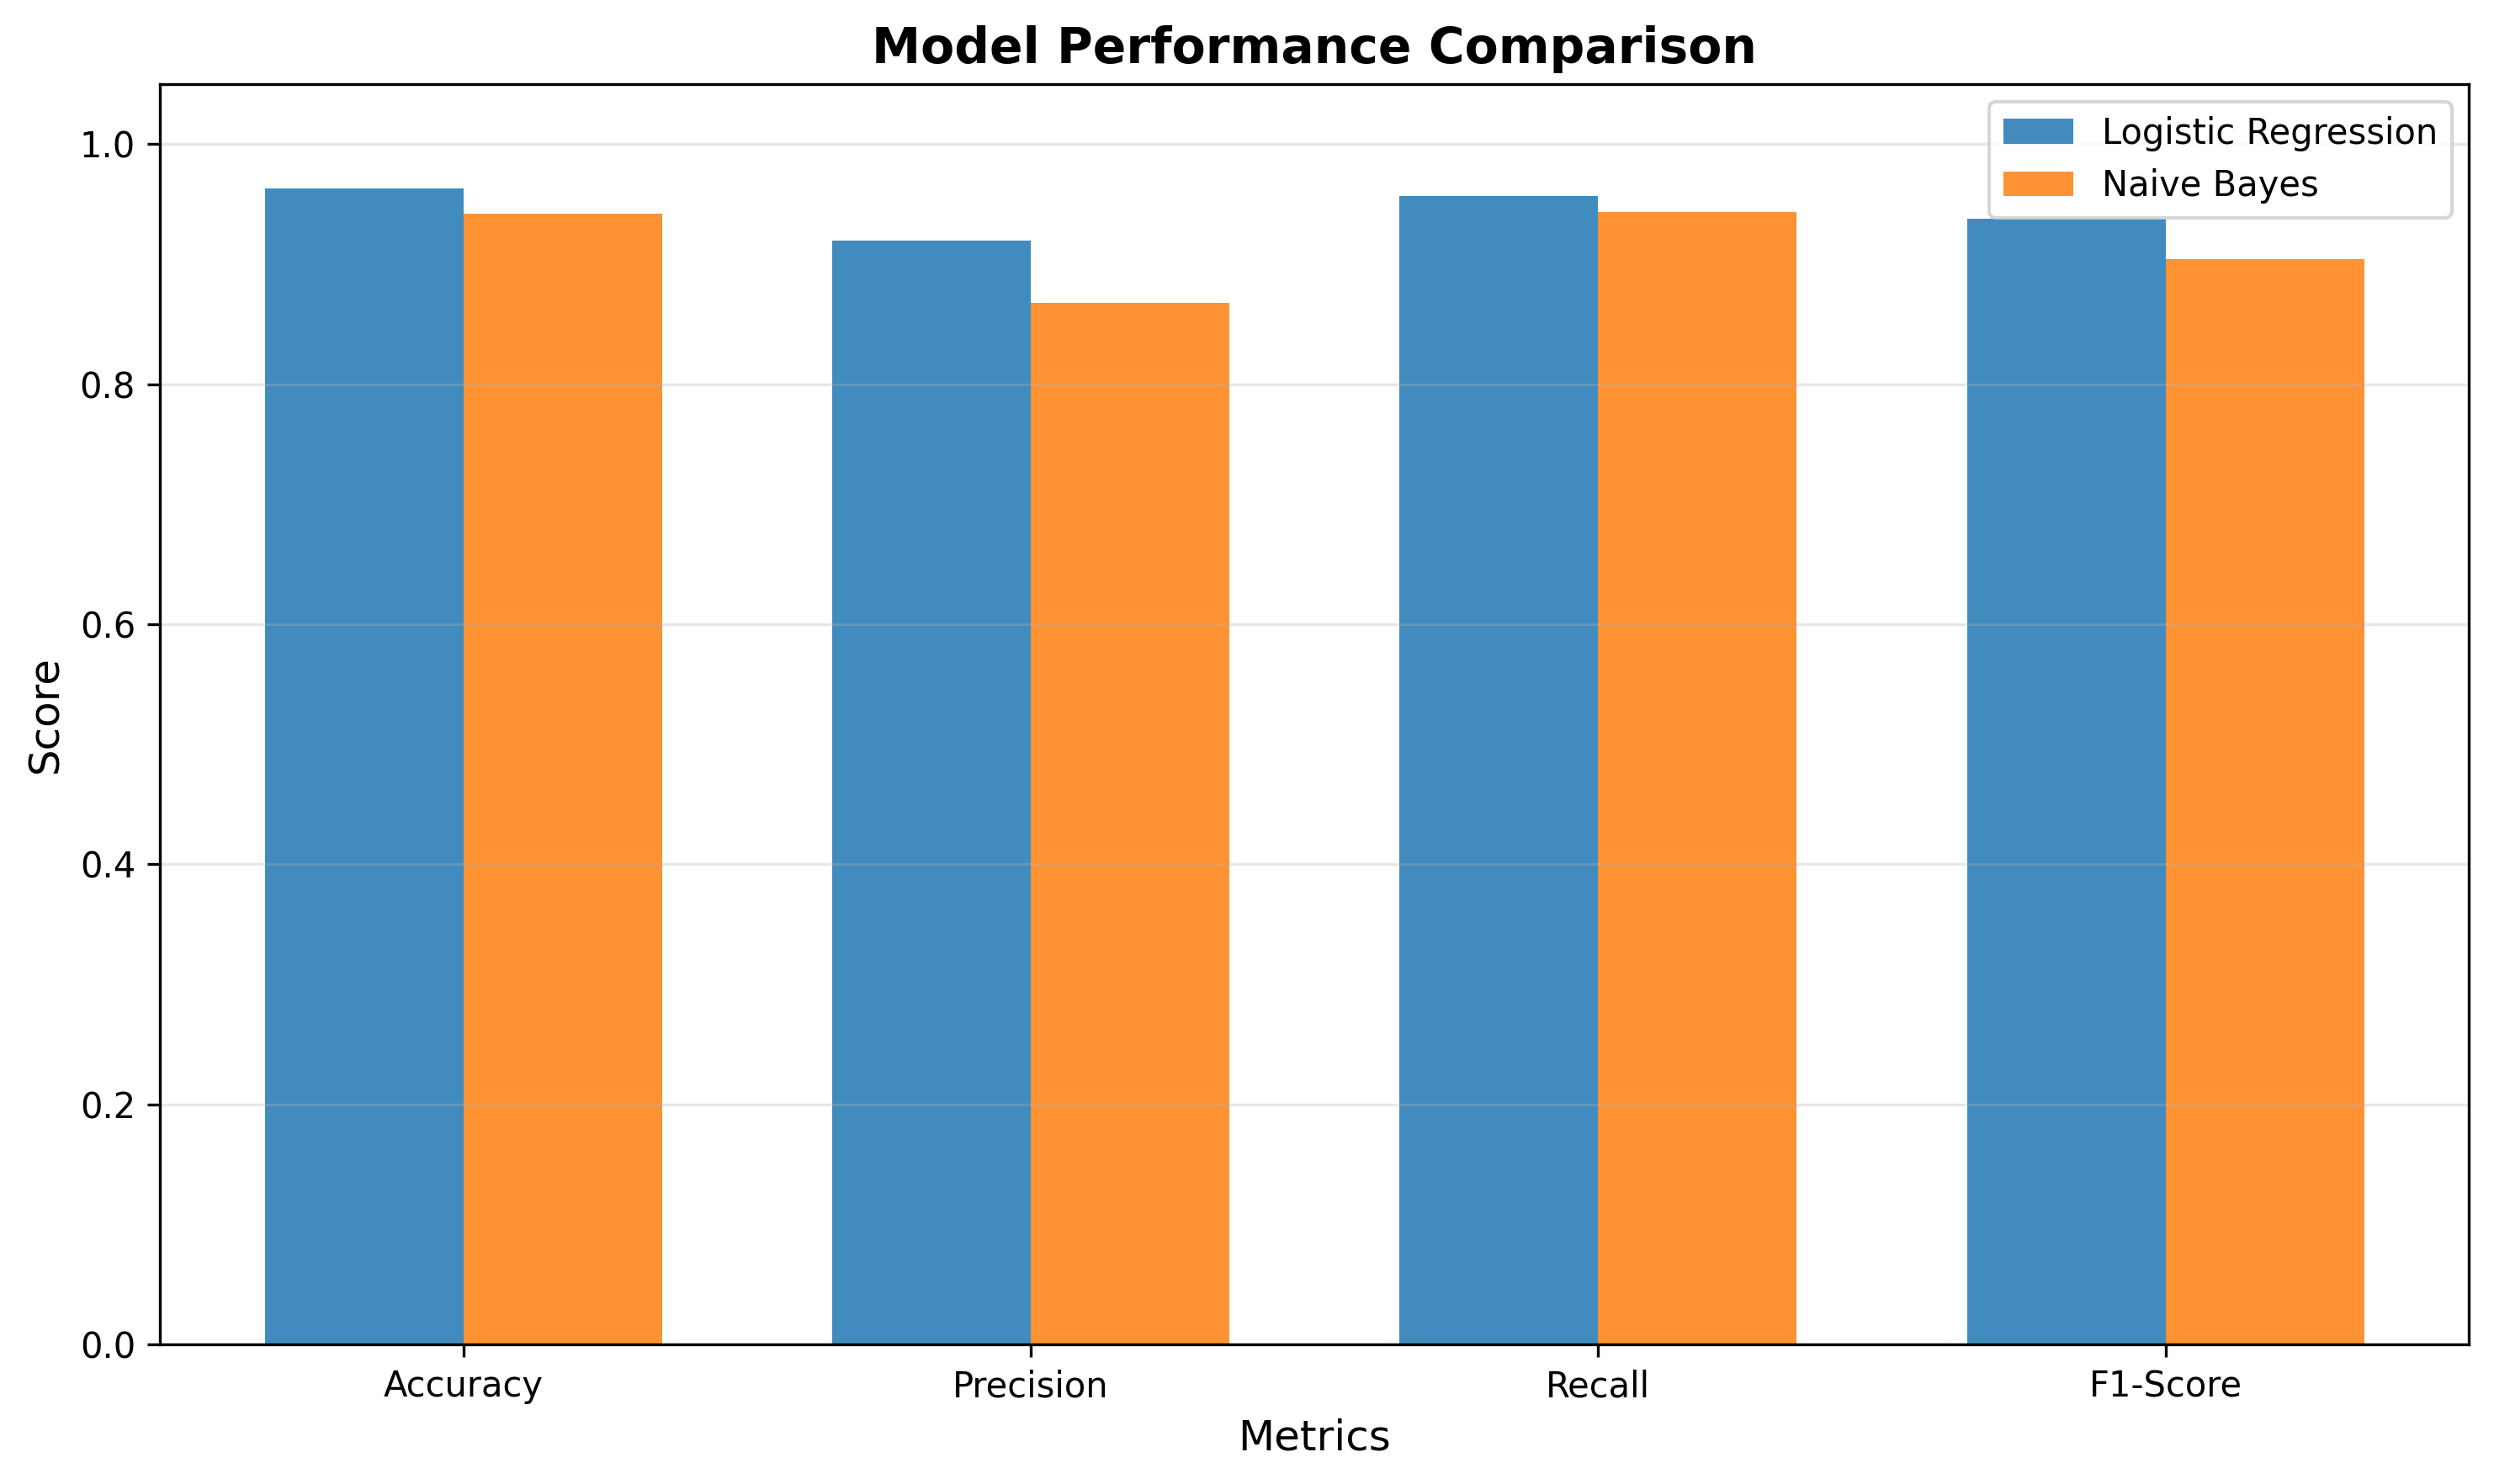
\includegraphics[width=0.48\textwidth]{figures/q1_model_comparison_bar.png}
\caption{Metric-level comparison for Q1 models.}
\label{fig:q1-bar}
\end{figure}

Figure~\ref{fig:q1-bar} summarizes model differences compactly and is consistent with the numerical table.

\subsection{Why Logistic Regression Wins Here}

Three factors explain the observed superiority of Logistic Regression:
\begin{enumerate}
    \item \textbf{Correlated lexical features:} words in real emails are not conditionally independent, violating Naive Bayes assumptions.
    \item \textbf{Discriminative optimization:} Logistic Regression optimizes a direct classification objective.
    \item \textbf{Feature normalization and gradient training:} stable optimization improves calibration on dense high-dimensional vectors.
\end{enumerate}

Naive Bayes still offers advantages in simplicity and training speed, but in this setting accuracy-oriented performance favors the discriminative model.

\section{Question 2: URL Feature Engineering and Modeling}

\subsection{Dataset Preparation}

The URL dataset contains 11,430 samples, balanced between \texttt{phishing} and \texttt{legitimate}. Labels are normalized to $\{0,1\}$ using explicit mapping rules. The balanced distribution enables cleaner interpretation of precision-recall behavior without severe class prior skew.

\subsection{Feature Set A: Structural Features}

The first configuration extracts low-cost structural counts directly from raw strings:
\begin{itemize}
    \item Number of dots,
    \item Number of slashes,
    \item Number of hyphens.
\end{itemize}

These attributes approximate URL complexity and segmentation patterns that are often associated with obfuscation \cite{chandrasekaran2006phishing}.

\subsection{Feature Set B: Statistical/Content Features}

The second configuration adds quantitative content signals:
\begin{itemize}
    \item Total URL length,
    \item Ratio of numeric characters,
    \item Longest alphabetic token length.
\end{itemize}

These features capture suspicious patterns such as excessive length and digit-heavy strings frequently observed in malicious links \cite{ma2011learning,aburrous2010intelligent}.

\subsection{Feature Set C: Creative Handcrafted Features}

The creative feature set introduces security-motivated indicators:
\begin{itemize}
    \item IP-based host usage,
    \item Presence of '@', '-', and percent encoding,
    \item Suspicious terms (e.g., \texttt{verify}, \texttt{login}, \texttt{secure}),
    \item HTTPS usage,
    \item Subdomain depth and path structure statistics.
\end{itemize}

Domain decomposition relies on \texttt{tldextract} \cite{tldextract} to separate subdomain/domain/suffix consistently.

\subsection{Feature Set D: Combined Features}

The final configuration concatenates structural, statistical, and creative features. This fusion tests whether complementary signals from multiple URL perspectives improve separability.

\subsection{Modeling Protocol for Q2}

For each feature set:
\begin{enumerate}
    \item Split data into 80\% train and 20\% test, with guarded stratification.
    \item Train Logistic Regression with standard scaling.
    \item Train Gaussian Naive Bayes for continuous-valued features.
    \item Evaluate using Accuracy, Precision, Recall, and F1-score.
\end{enumerate}

Unlike Question 1 (from-scratch requirement), Q2 intentionally uses library implementations to focus on feature-design impact.

\subsection{Visualization Coverage}

The notebook exports eight Q2 figures to support multi-angle interpretation:
\begin{itemize}
    \item Structural distributions,
    \item Combined-feature correlation heatmap,
    \item Structural boxplots by class,
    \item Pairplot of sampled features,
    \item Top mean absolute correlations,
    \item ROC comparison for combined features,
    \item Precision-Recall curve for combined Logistic Regression,
    \item Logistic Regression coefficient importance.
\end{itemize}

\section{Question 2: Results and Comparative Analysis}

\subsection{Performance Across Feature Sets}

Tables~\ref{tab:q2-lr} and \ref{tab:q2-nb} summarize model performance for each feature configuration.

\begin{table}[H]
\centering
\caption{Logistic Regression performance across Q2 feature sets}
\label{tab:q2-lr}
\begin{tabular}{lcccc}
\toprule
Feature set & Acc & Prec & Rec & F1 \\
\midrule
Structural only          & 0.6763 & 0.7042 & 0.6080 & 0.6526 \\
Statistical/content      & 0.6518 & 0.6974 & 0.5363 & 0.6063 \\
Creative handcrafted     & 0.7310 & 0.7750 & 0.6509 & 0.7076 \\
All combined             & 0.7857 & 0.8315 & 0.7165 & 0.7697 \\
\bottomrule
\end{tabular}
\end{table}

\begin{table}[H]
\centering
\caption{Gaussian Naive Bayes performance across Q2 feature sets}
\label{tab:q2-nb}
\begin{tabular}{lcccc}
\toprule
Feature set & Acc & Prec & Rec & F1 \\
\midrule
Structural only          & 0.6824 & 0.8243 & 0.4637 & 0.5935 \\
Statistical/content      & 0.6444 & 0.7696 & 0.4121 & 0.5368 \\
Creative handcrafted     & 0.6601 & 0.9621 & 0.3333 & 0.4951 \\
All combined             & 0.7227 & 0.9442 & 0.4733 & 0.6305 \\
\bottomrule
\end{tabular}
\end{table}

The combined feature configuration is best for both models. Logistic Regression achieves the strongest overall balance, while Naive Bayes tends to exhibit very high precision with noticeably lower recall.

\subsection{Combined-Model Error Decomposition}

Because combined features provide the best headline performance, we inspect their confusion structure directly in Table~\ref{tab:q2-combined-diagnostics}.

\begin{table}[H]
\centering
\caption{Detailed diagnostics on combined features (Q2)}
\label{tab:q2-combined-diagnostics}
\scriptsize
\setlength{\tabcolsep}{3.5pt}
\begin{tabular}{lcc}
\toprule
Metric & Logistic Regression & Gaussian NB \\
\midrule
TN / FP / FN / TP & 977 / 166 / 324 / 819 & 1111 / 32 / 602 / 541 \\
Specificity & 0.8548 & 0.9720 \\
Balanced Accuracy & 0.7857 & 0.7227 \\
MCC & 0.5768 & 0.5138 \\
False Positive Rate & 0.1452 & 0.0280 \\
False Negative Rate & 0.2835 & 0.5267 \\
F1 95\% CI (bootstrap) & [0.7470, 0.7882] & [0.6024, 0.6576] \\
\bottomrule
\end{tabular}
\end{table}

The table clarifies a central tradeoff: Gaussian NB is much more conservative (very low FPR), but it misses a large fraction of true phishing URLs (high FNR). Logistic Regression accepts more false alarms yet recovers substantially more positives, yielding better balanced accuracy and F1.

\subsection{Relative Gain Analysis Across Feature Families}

To quantify feature-engineering value, we compare the best and weakest feature families:
\begin{itemize}
    \item Logistic Regression F1 improves from 0.6063 (statistical/content) to 0.7697 (combined), a +26.96\% relative gain.
    \item Logistic Regression recall improves from 0.5363 to 0.7165, a +33.61\% relative gain.
    \item Naive Bayes F1 improves from 0.5368 (statistical/content) to 0.6305 (combined), a +17.46\% relative gain.
    \item Naive Bayes recall improves from 0.4121 to 0.4733, a +14.85\% relative gain.
\end{itemize}

These improvements indicate that engineering richer feature views has larger impact than changing linear-probabilistic baseline type alone.

\subsection{Distributional and Correlation Insights}

\begin{figure}[H]
\centering
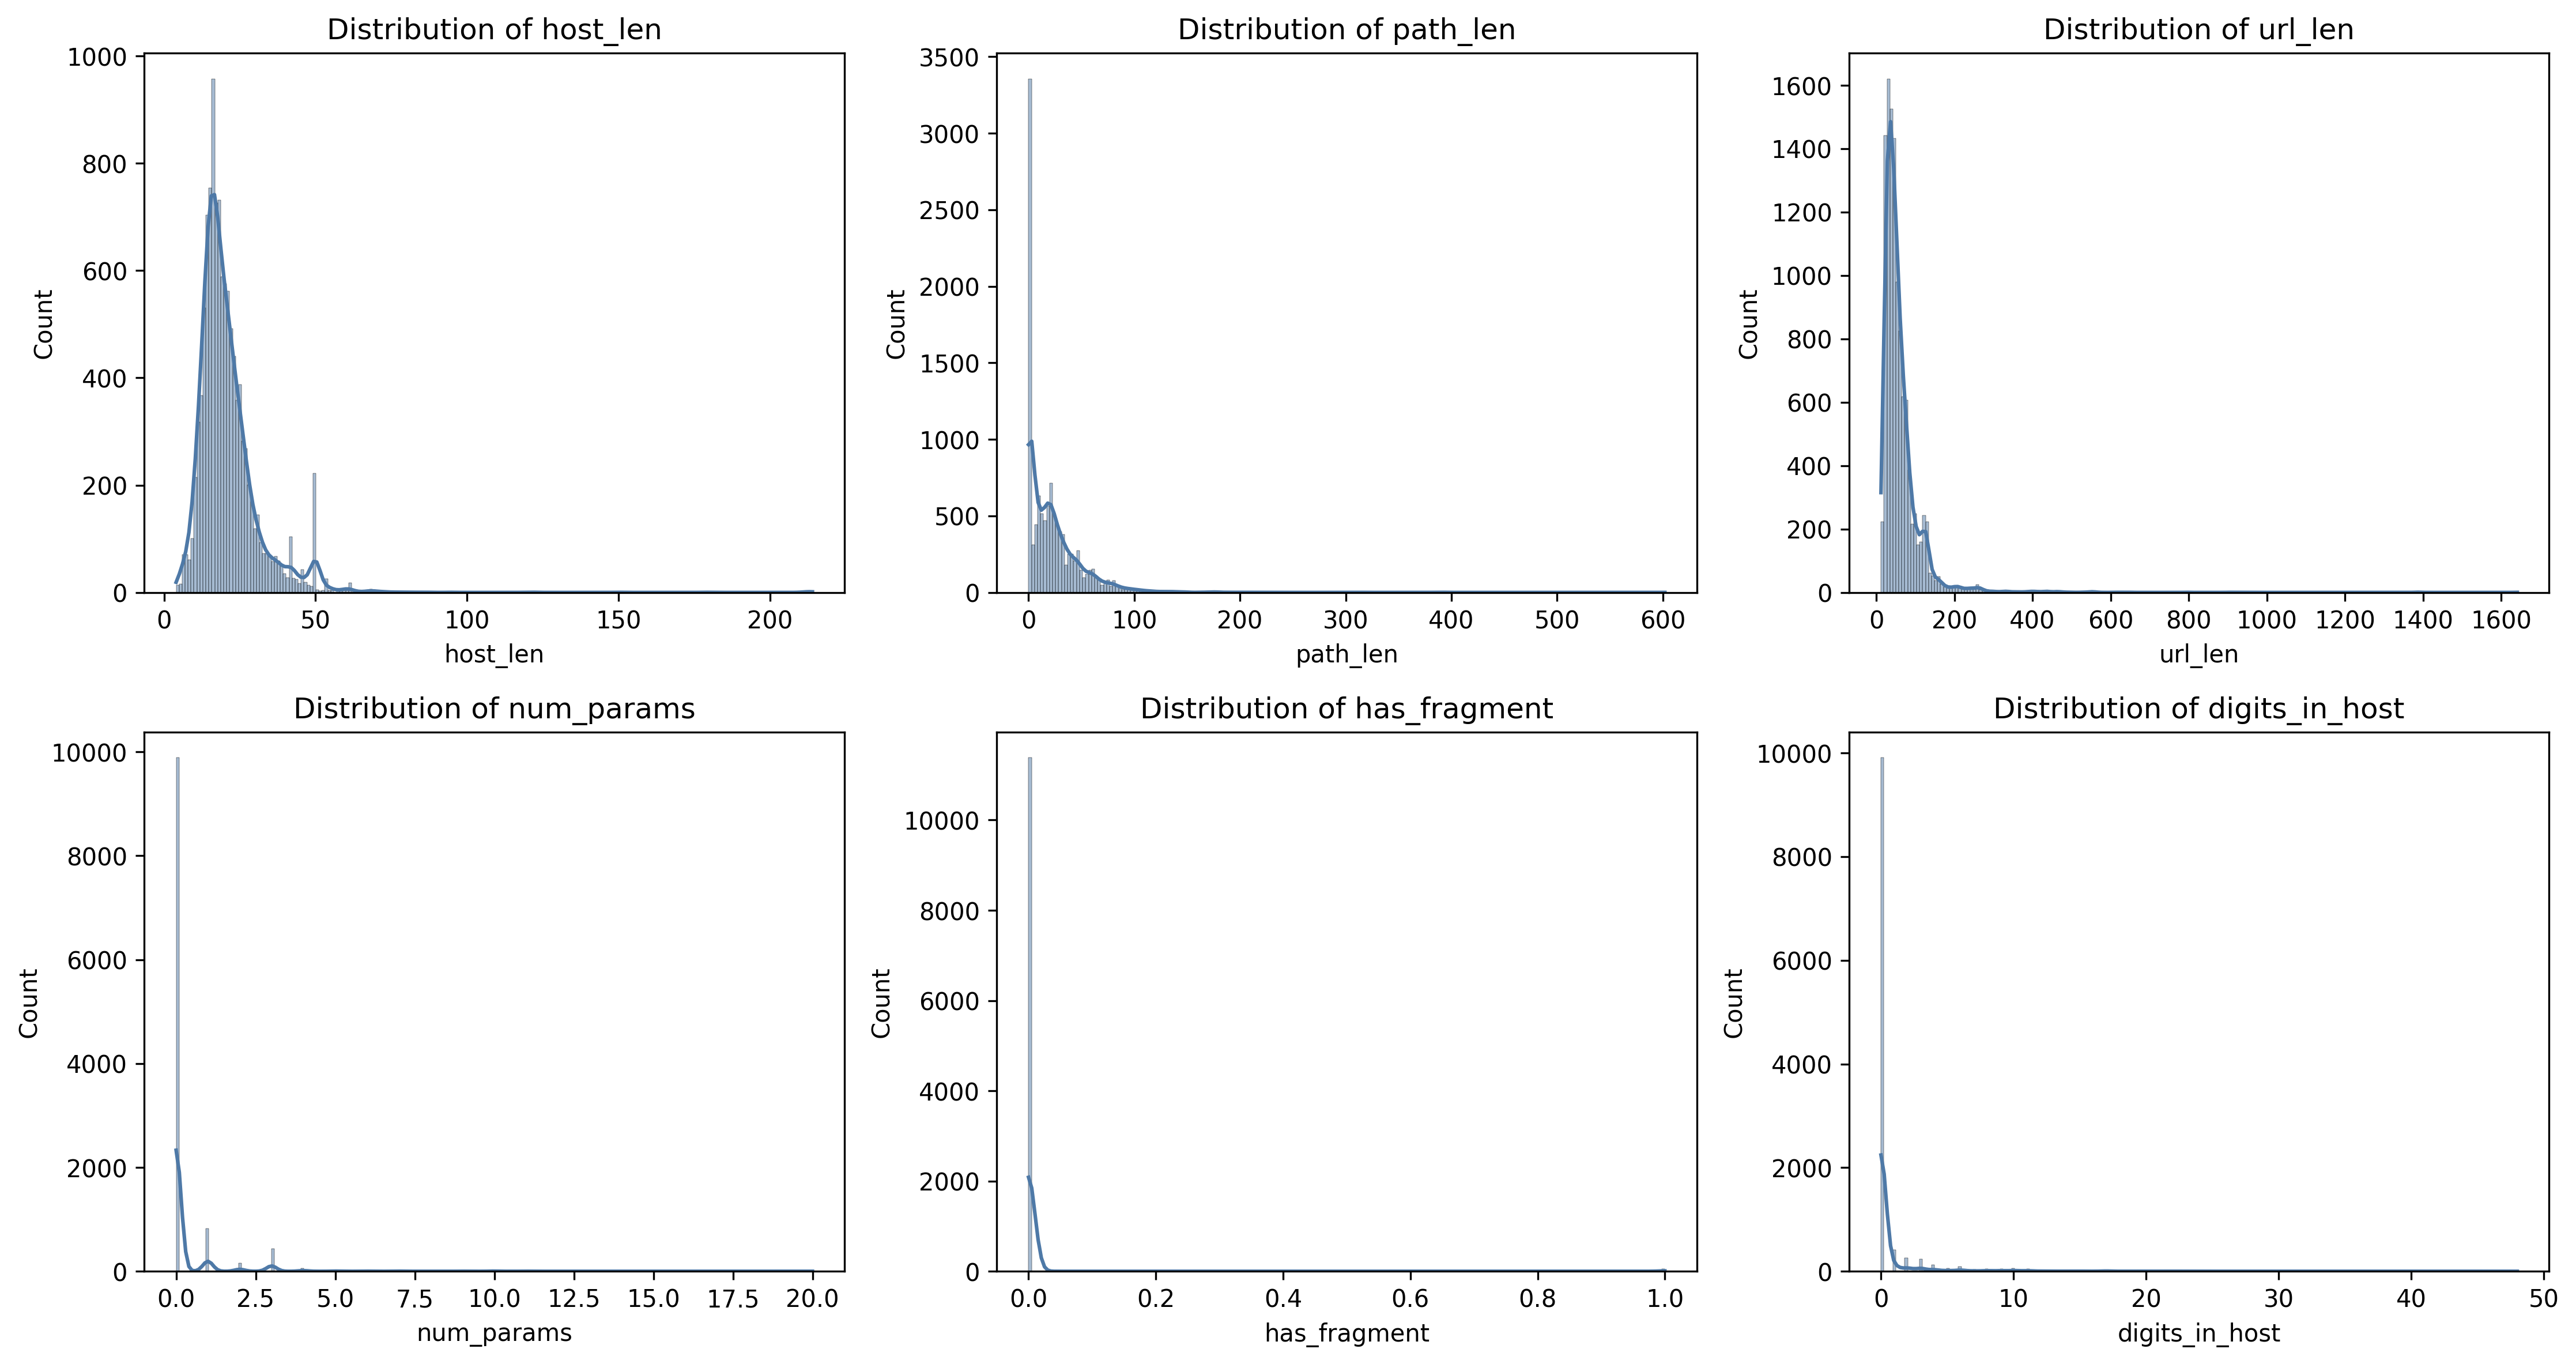
\includegraphics[width=0.48\textwidth]{figures/q2_structural_distributions.png}
\caption{Distributions of structural URL attributes.}
\label{fig:q2-struct-dist}
\end{figure}

\begin{figure}[H]
\centering
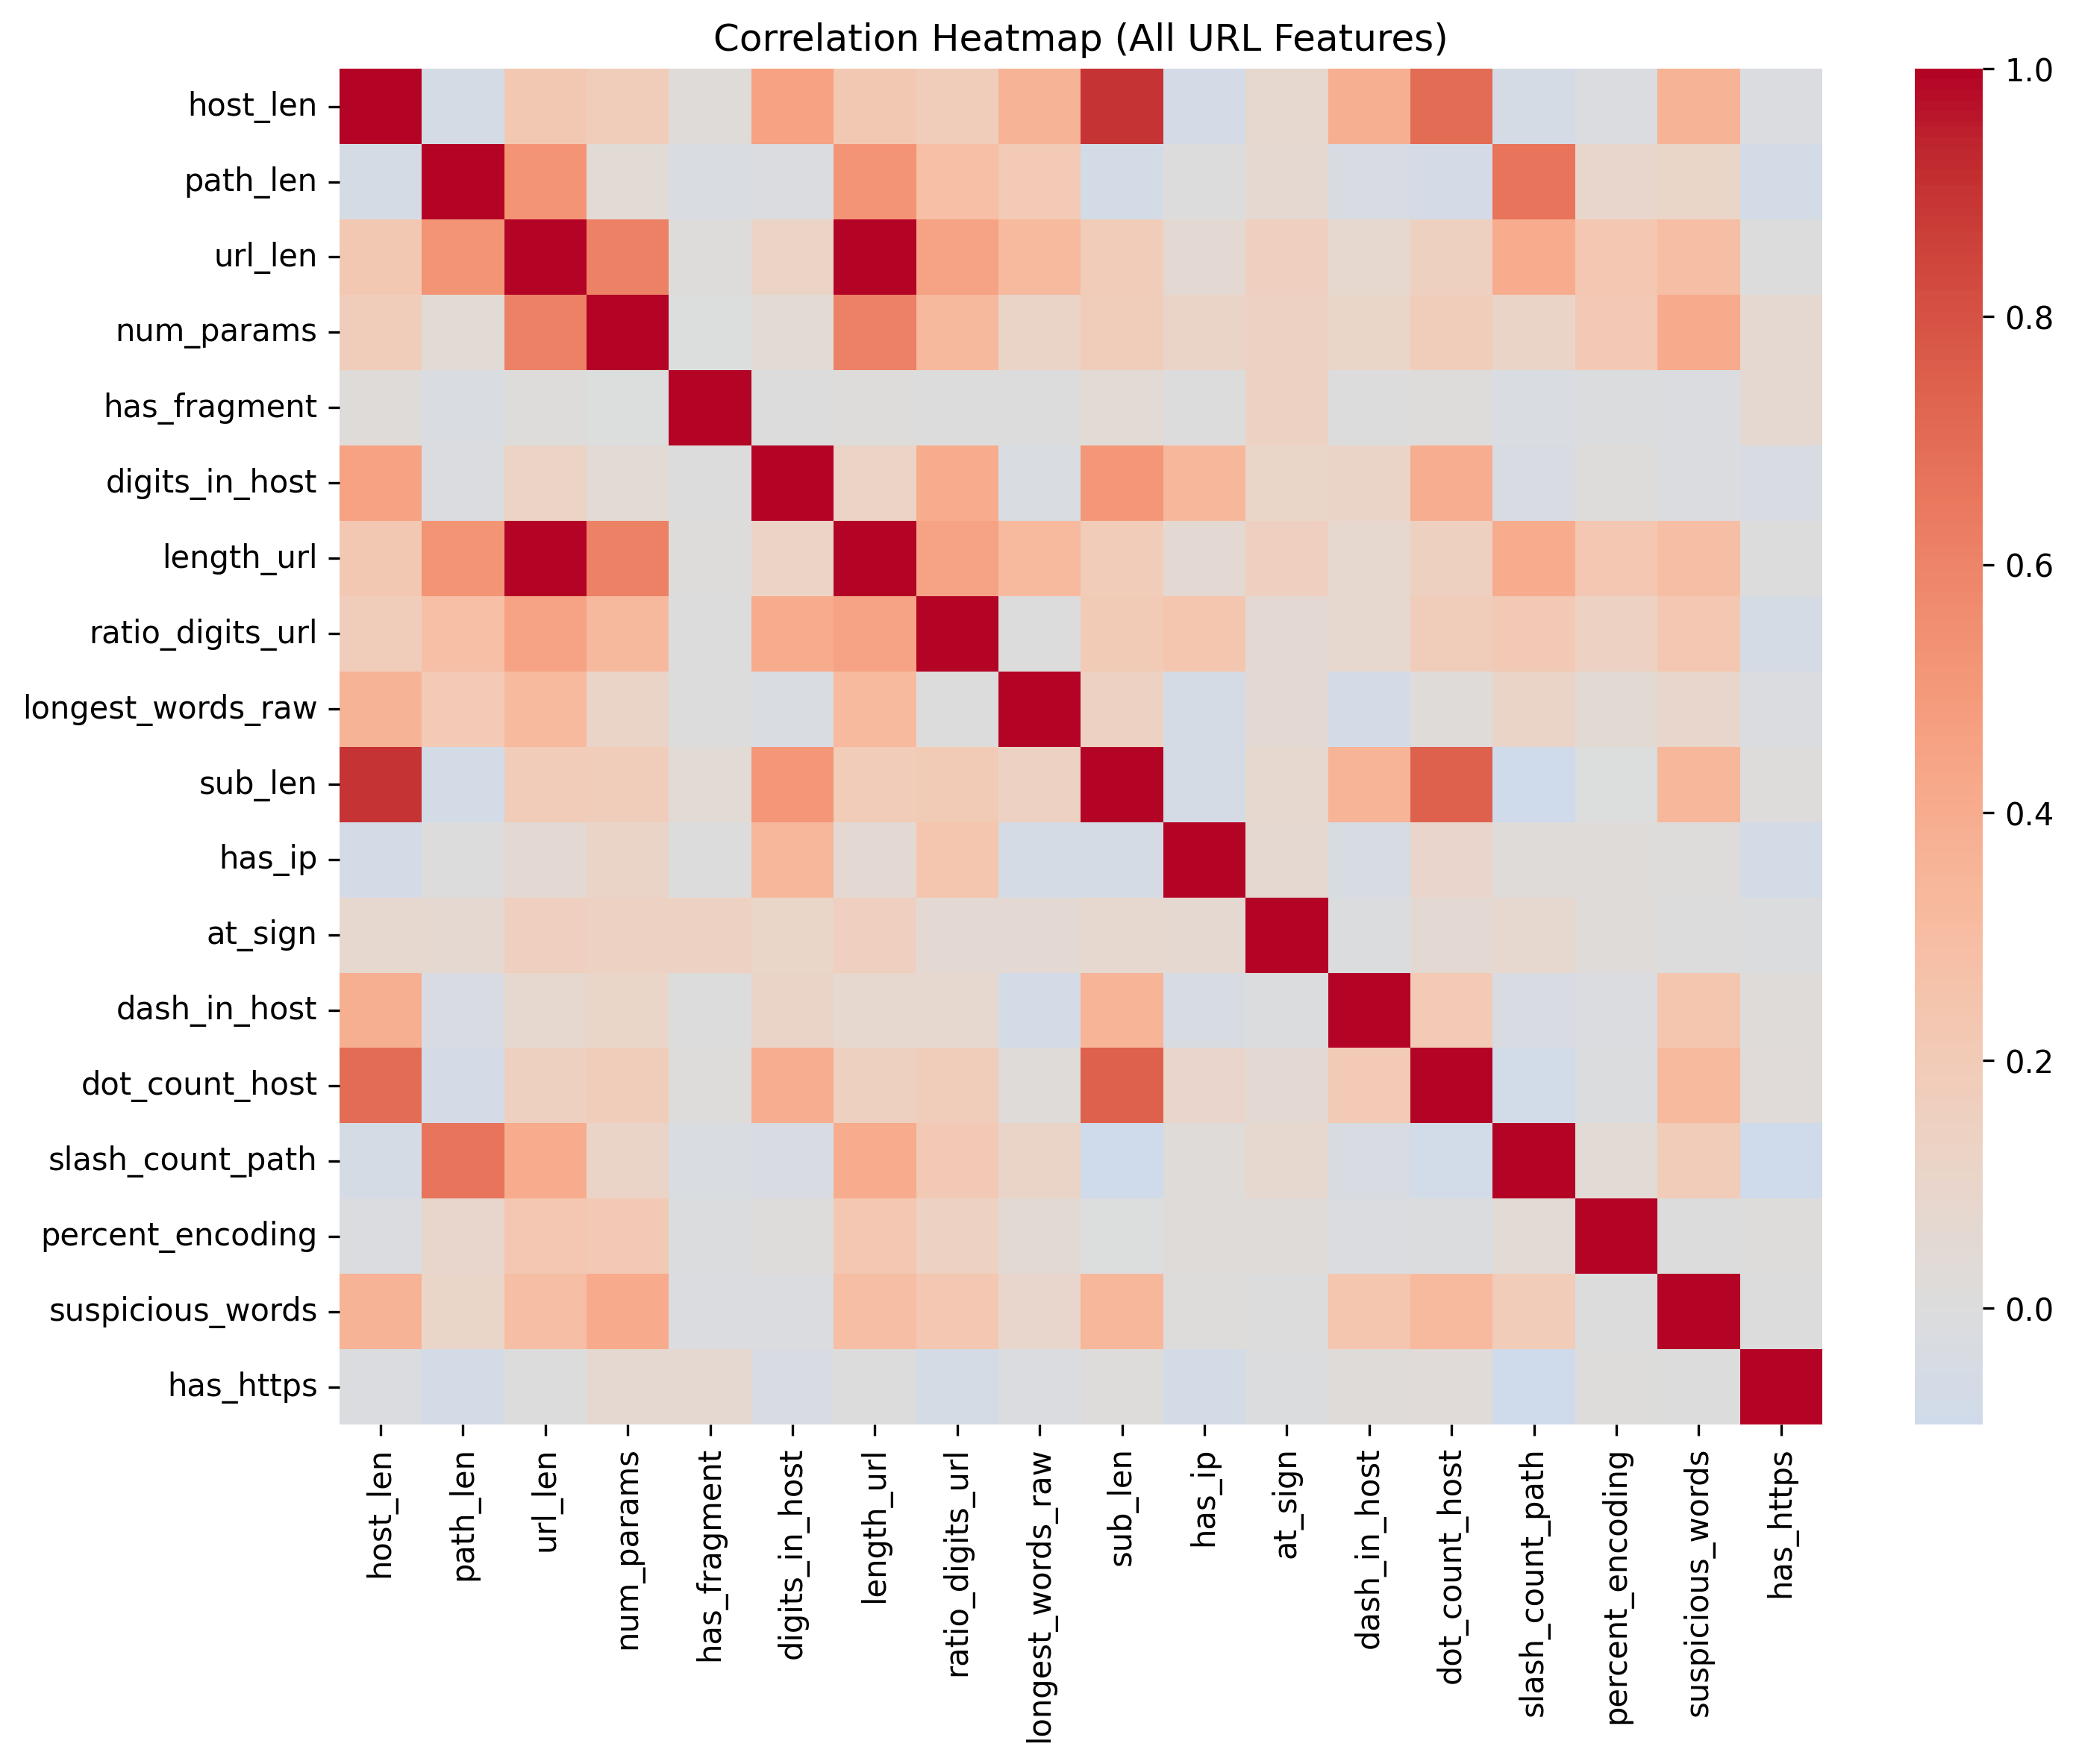
\includegraphics[width=0.48\textwidth]{figures/q2_correlation_heatmap_all_features.png}
\caption{Correlation heatmap of combined URL features.}
\label{fig:q2-corr}
\end{figure}

Figures~\ref{fig:q2-struct-dist} and \ref{fig:q2-corr} reveal moderate inter-feature dependency, indicating that combining views (length, host composition, token patterns) is likely to improve discriminative learning.

\begin{figure}[H]
\centering
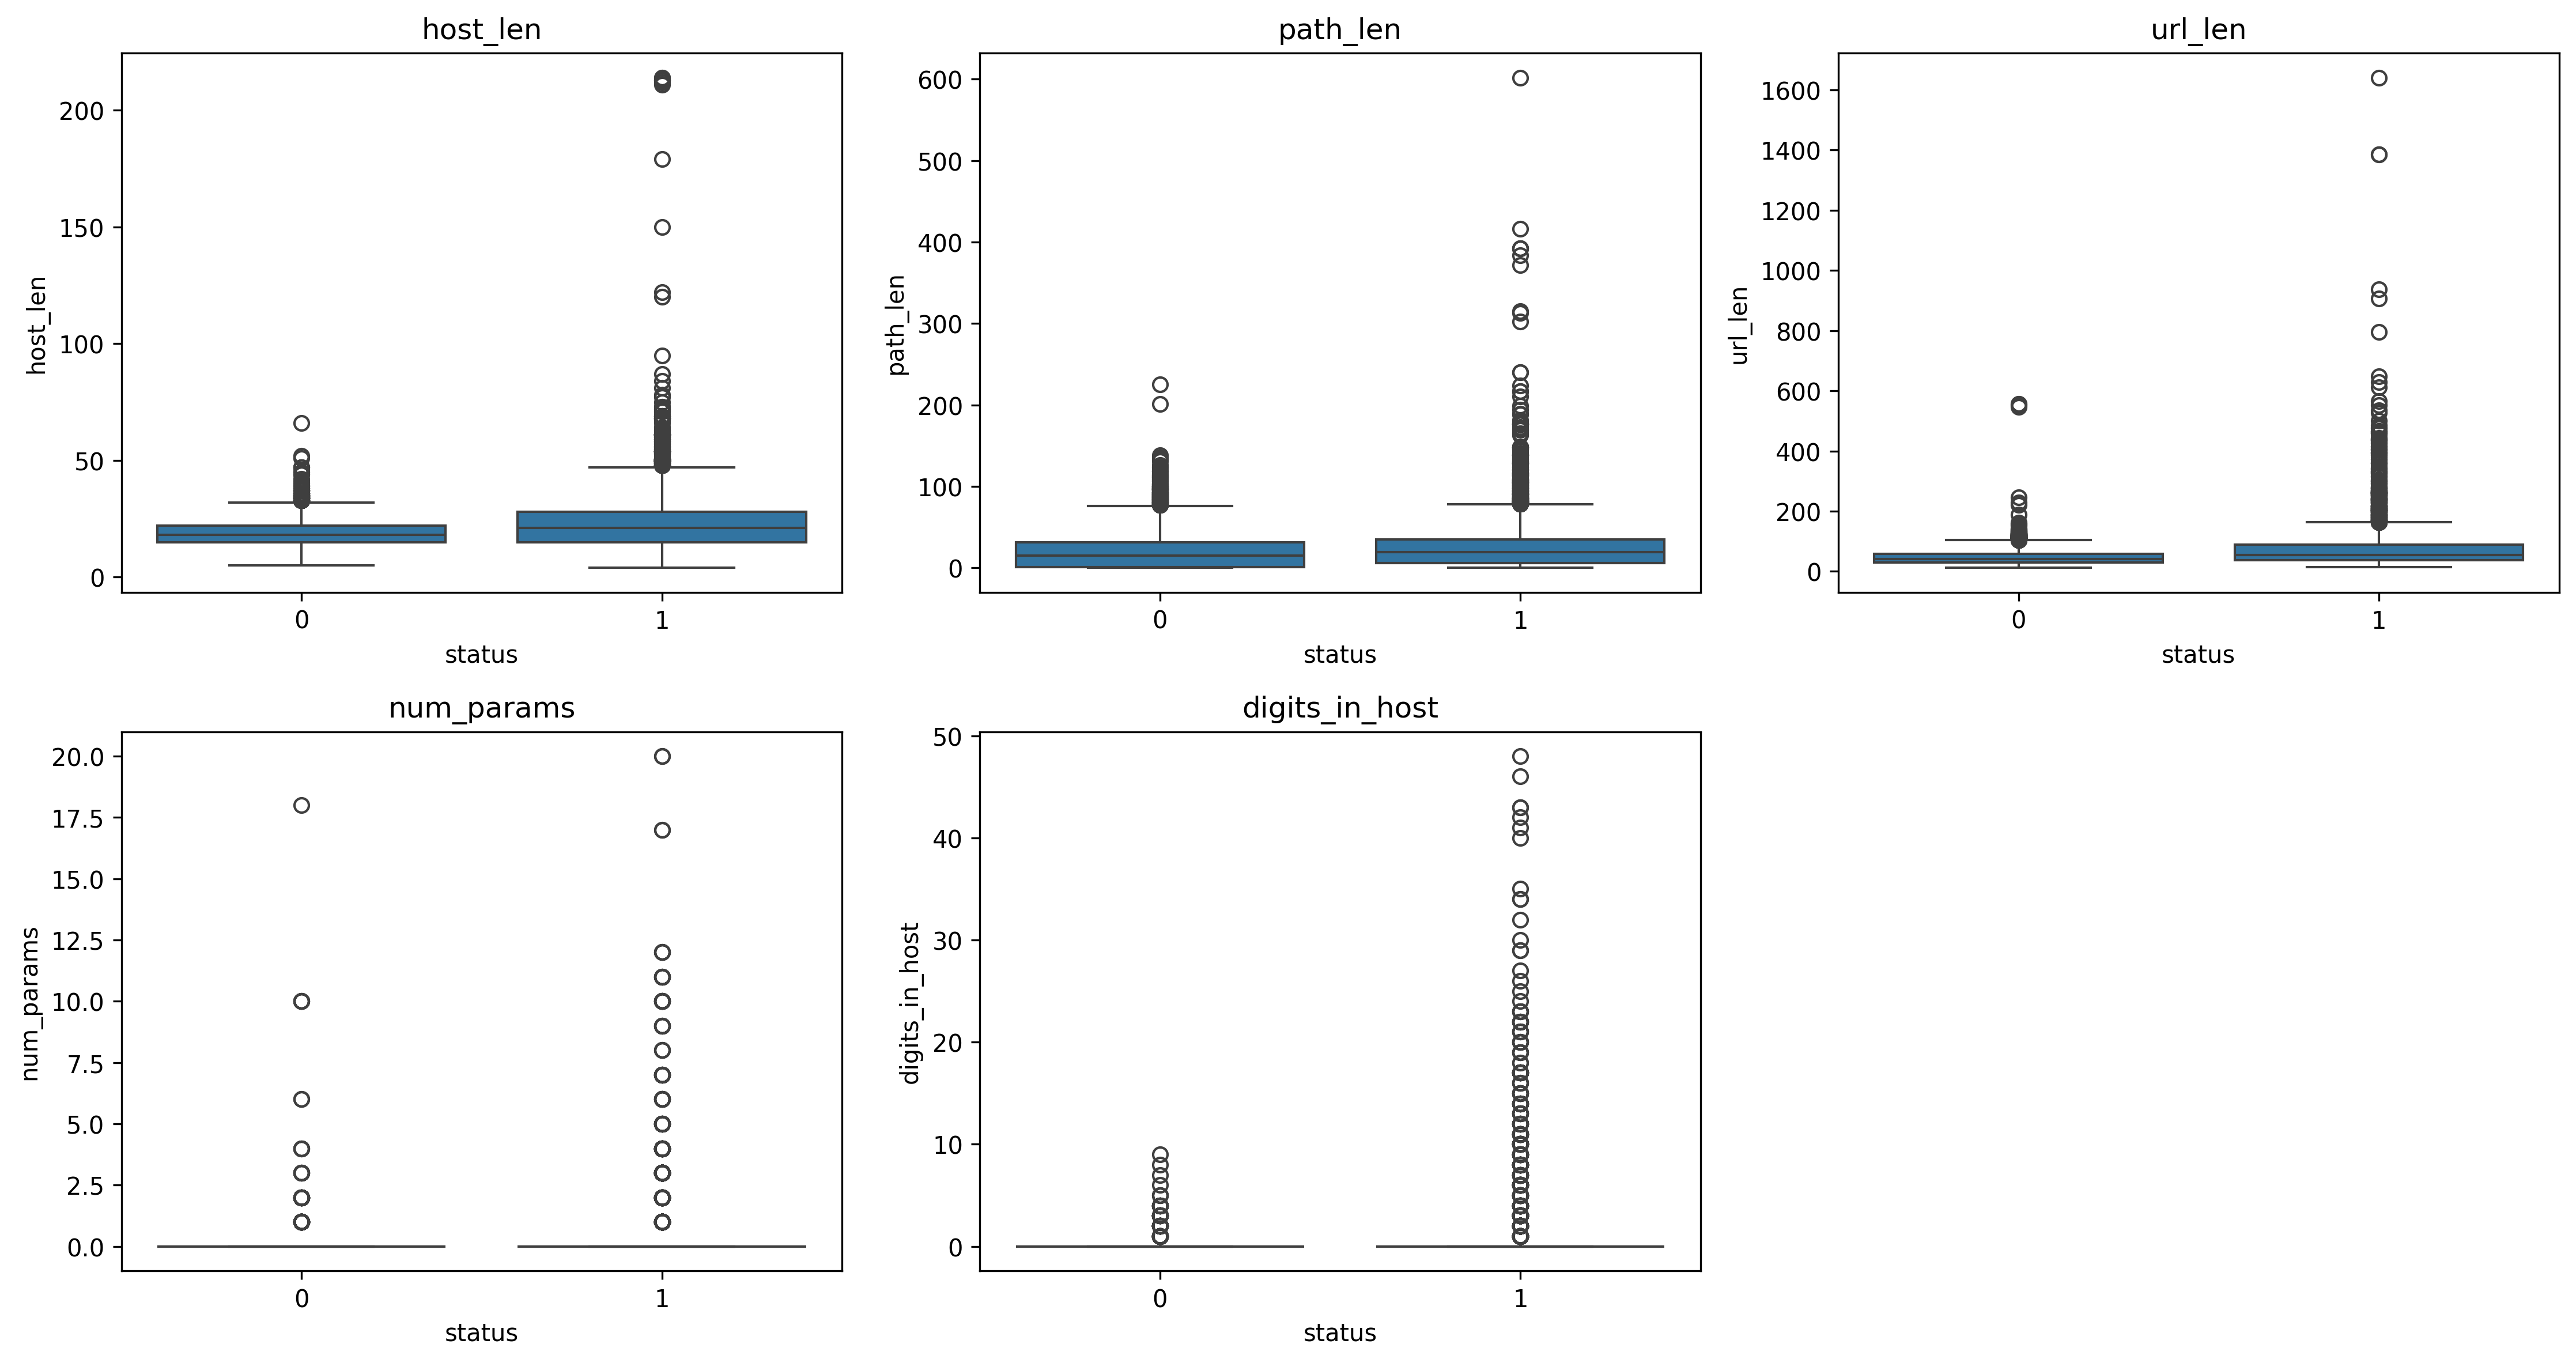
\includegraphics[width=0.48\textwidth]{figures/q2_structural_boxplots.png}
\caption{Structural feature separation by class label.}
\label{fig:q2-box}
\end{figure}

\begin{figure}[H]
\centering
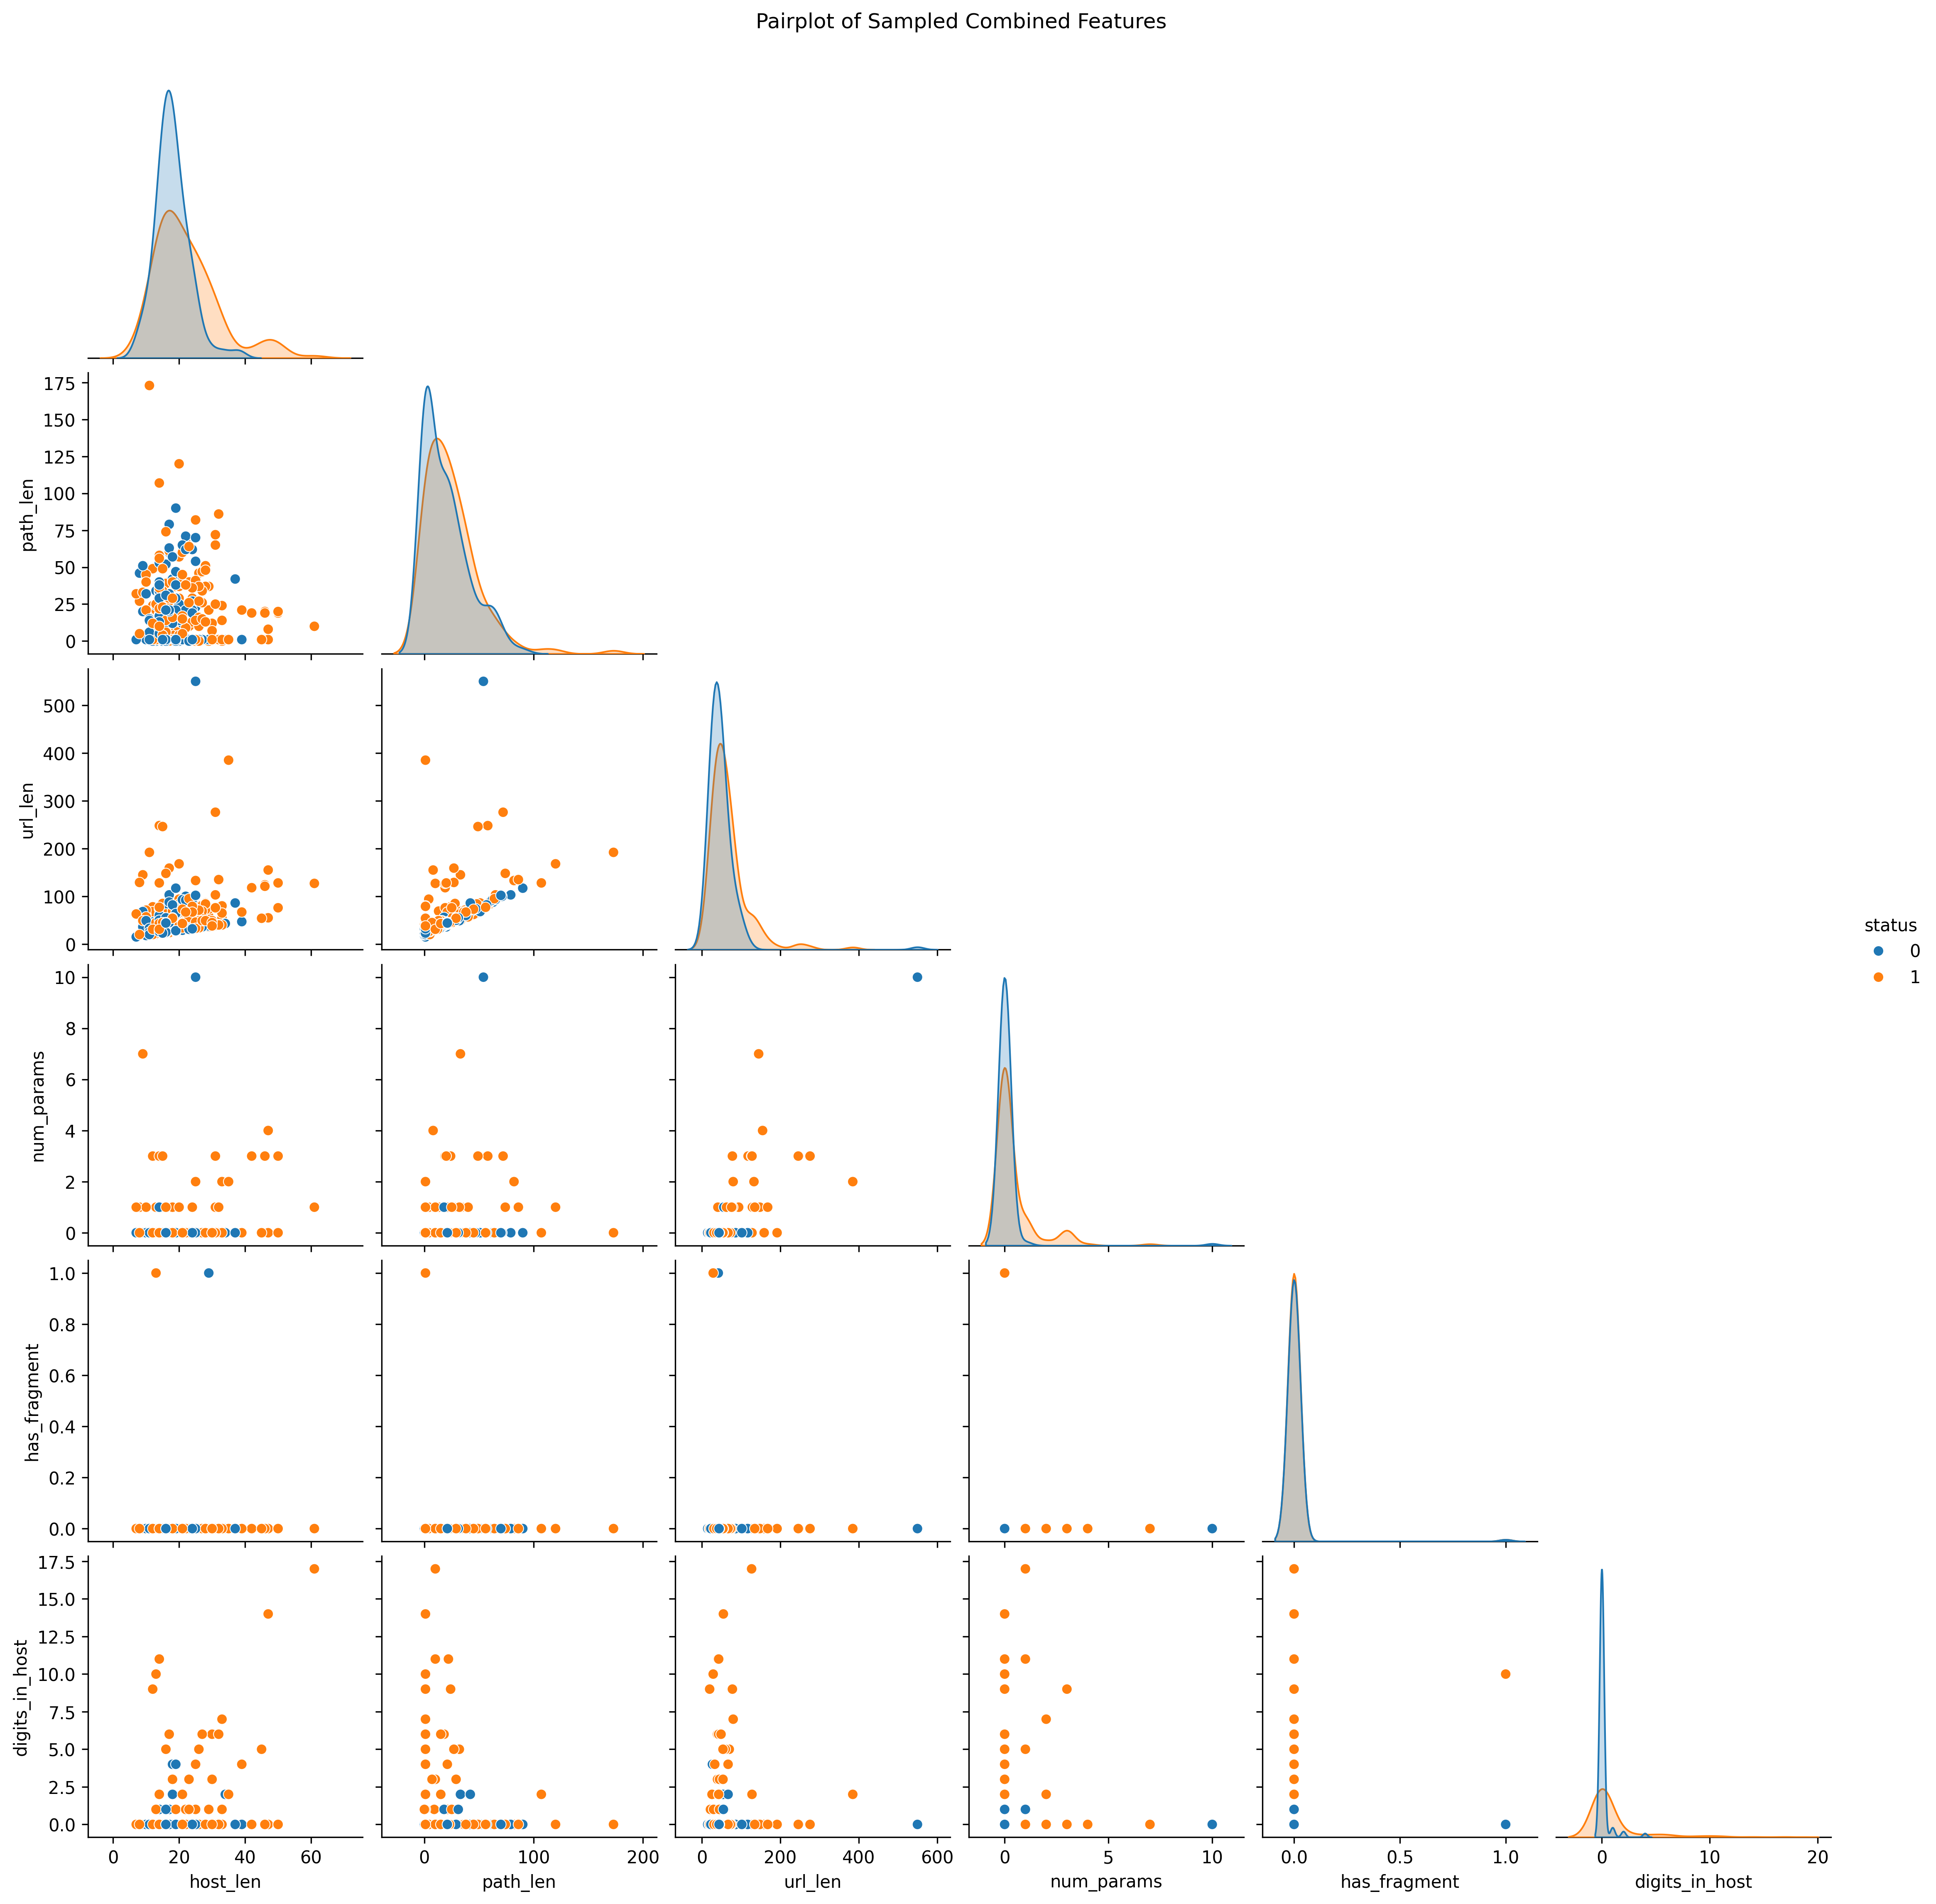
\includegraphics[width=0.48\textwidth]{figures/q2_pairplot_sample.png}
\caption{Pairwise view of sampled combined features.}
\label{fig:q2-pair}
\end{figure}

The boxplot and pairplot views in Figures~\ref{fig:q2-box} and \ref{fig:q2-pair} show partial class overlap but meaningful margin shifts in several dimensions, supporting the improvements observed in the combined setup.

\subsection{Feature Importance and Ranking Curves}

\begin{figure}[H]
\centering
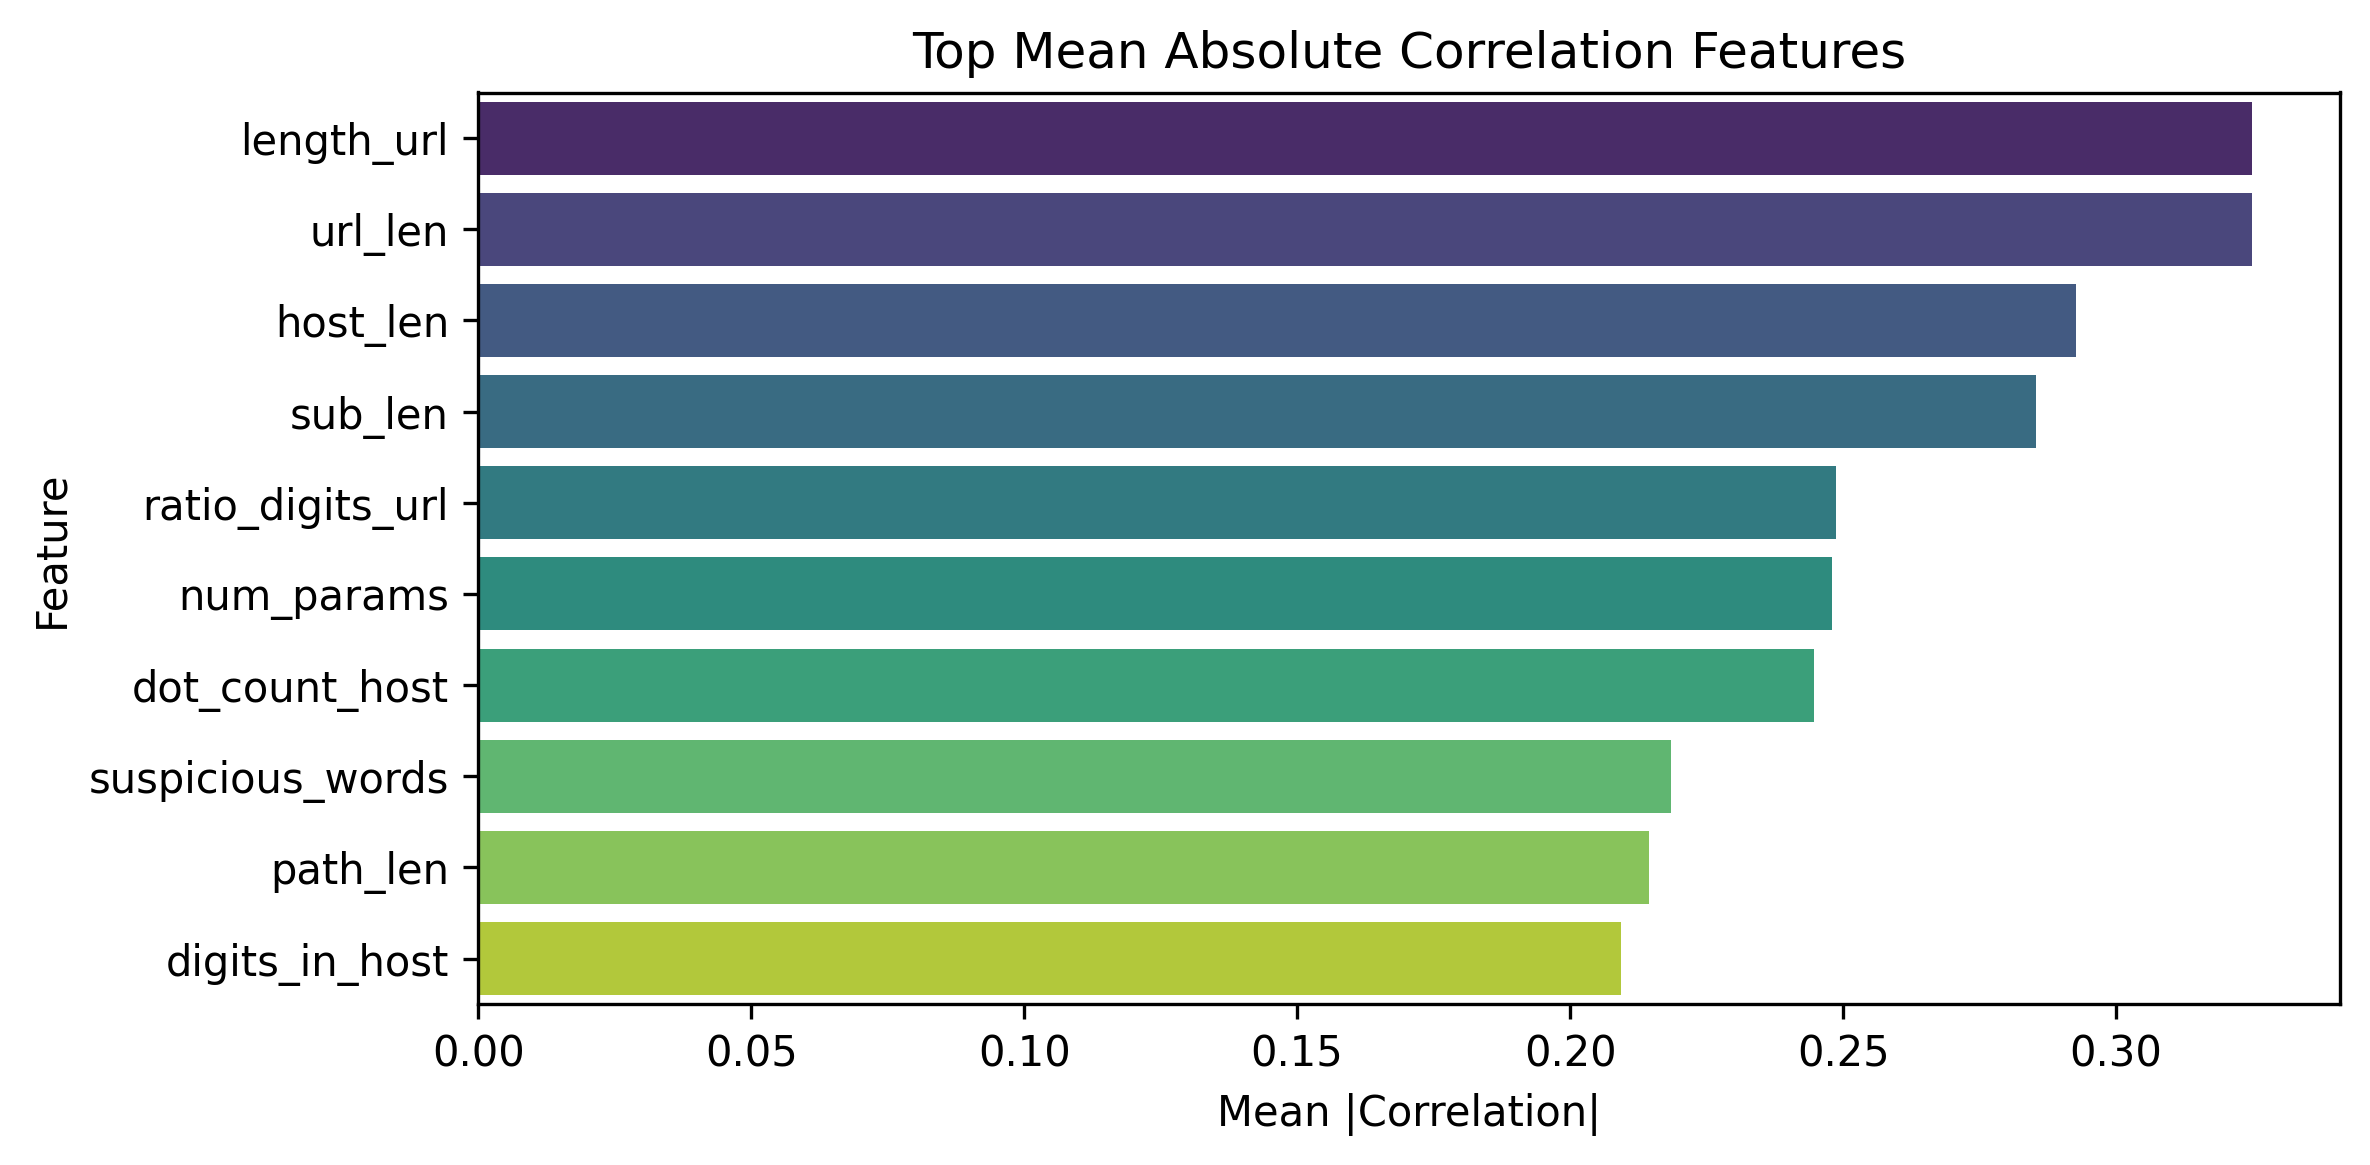
\includegraphics[width=0.48\textwidth]{figures/q2_top_mean_abs_correlations.png}
\caption{Top features by mean absolute correlation.}
\label{fig:q2-topcorr}
\end{figure}

\begin{figure}[H]
\centering
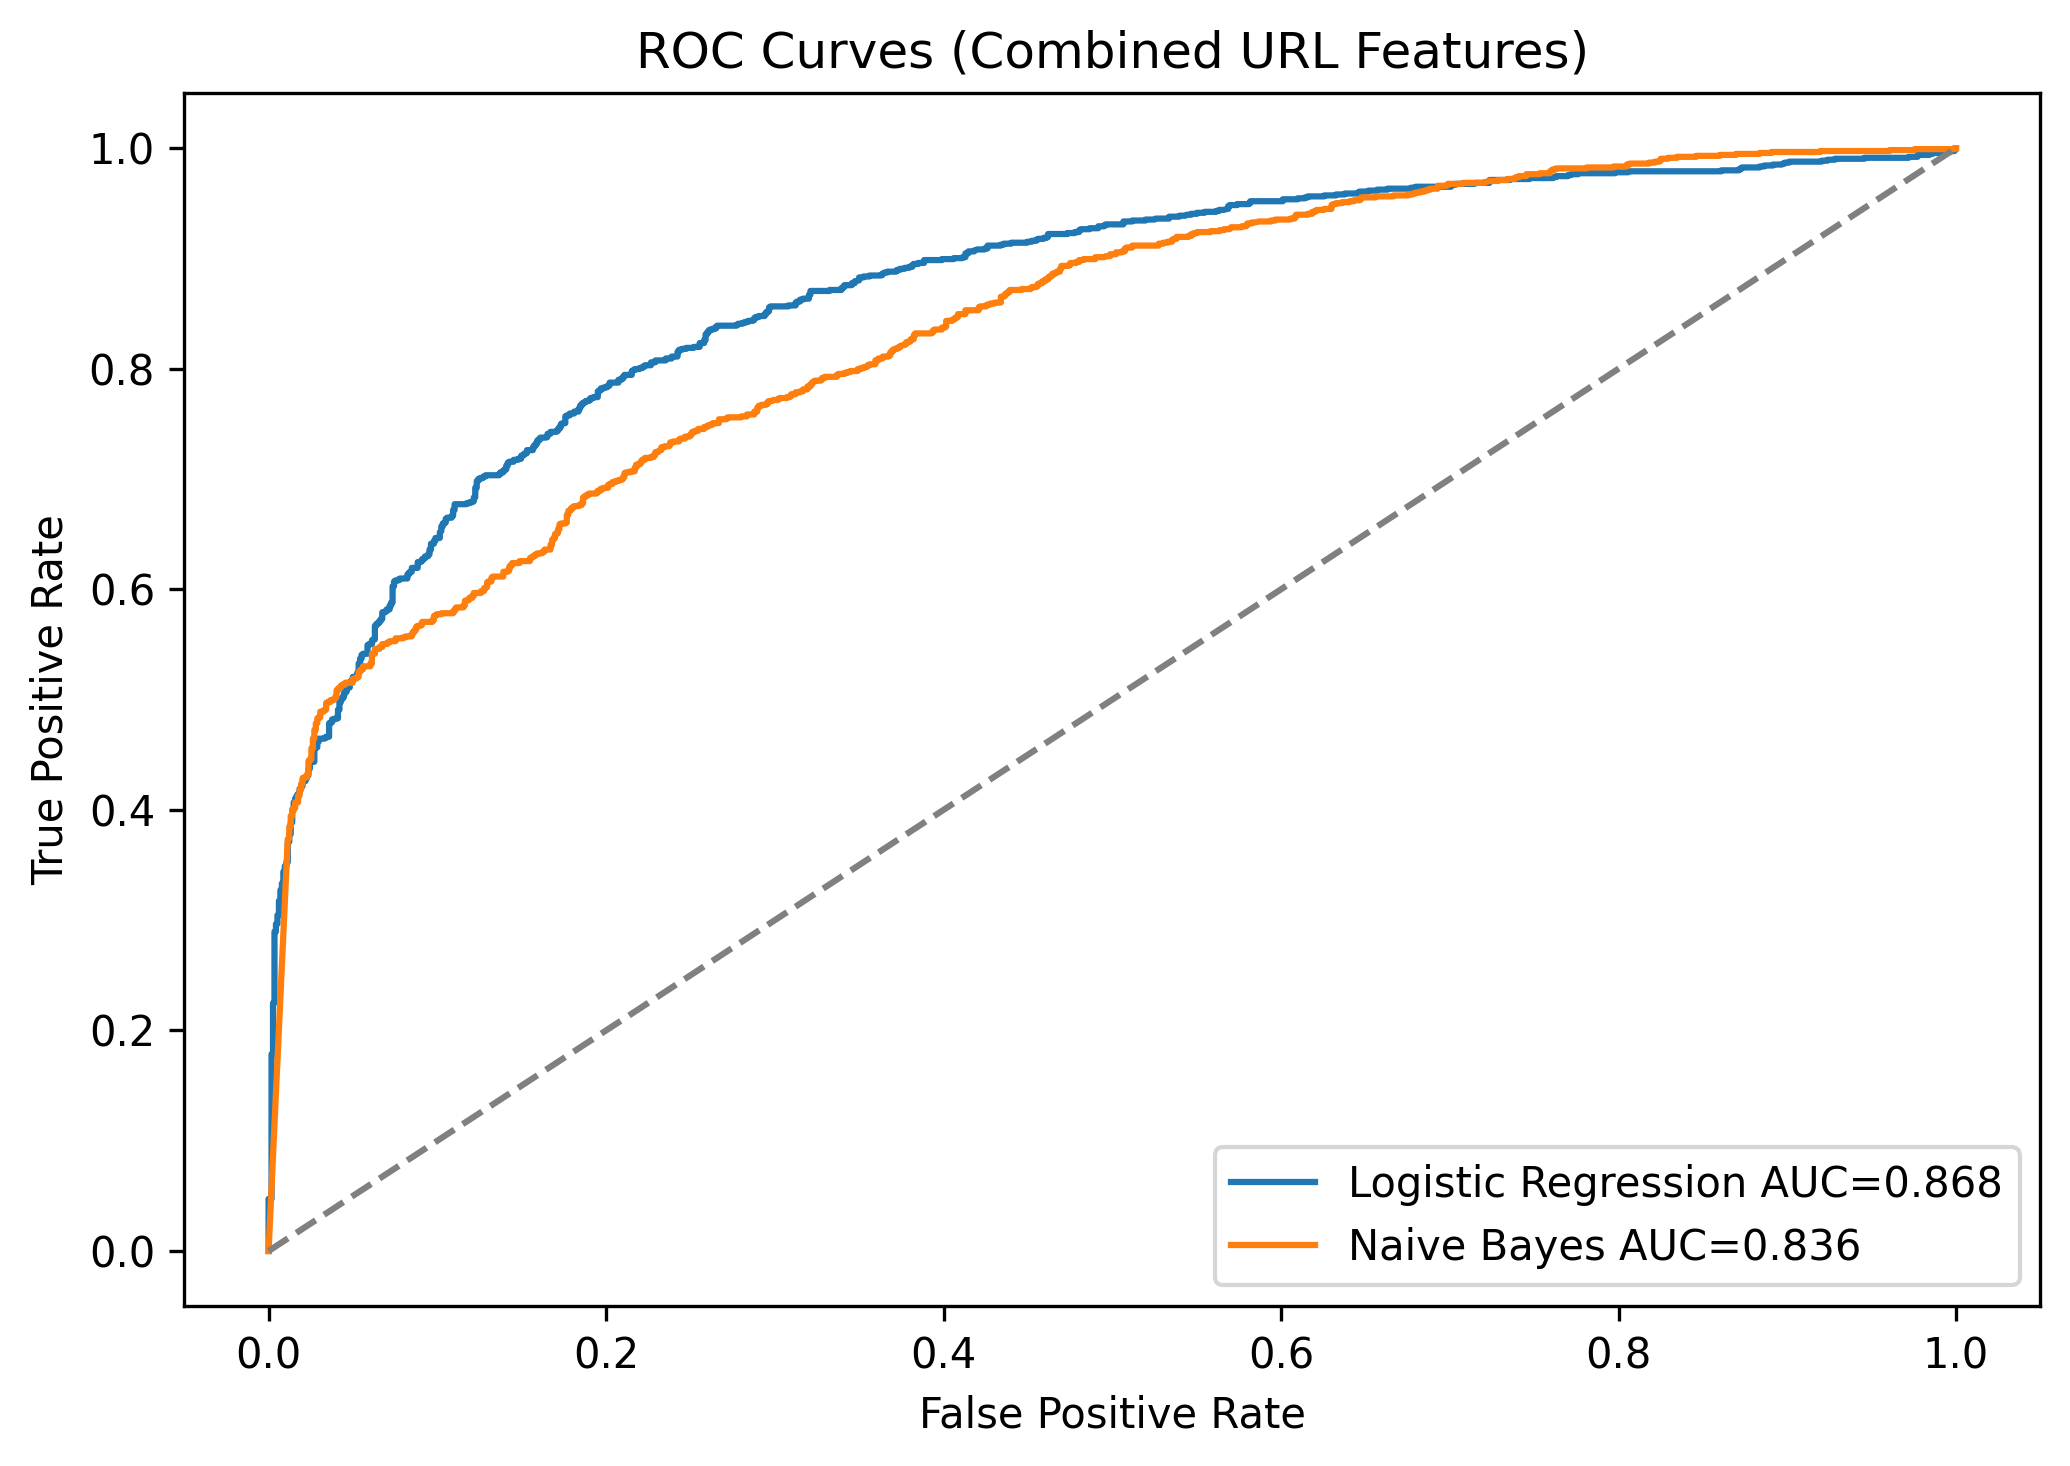
\includegraphics[width=0.48\textwidth]{figures/q2_roc_combined_features.png}
\caption{ROC comparison on combined features.}
\label{fig:q2-roc}
\end{figure}

\begin{figure}[H]
\centering
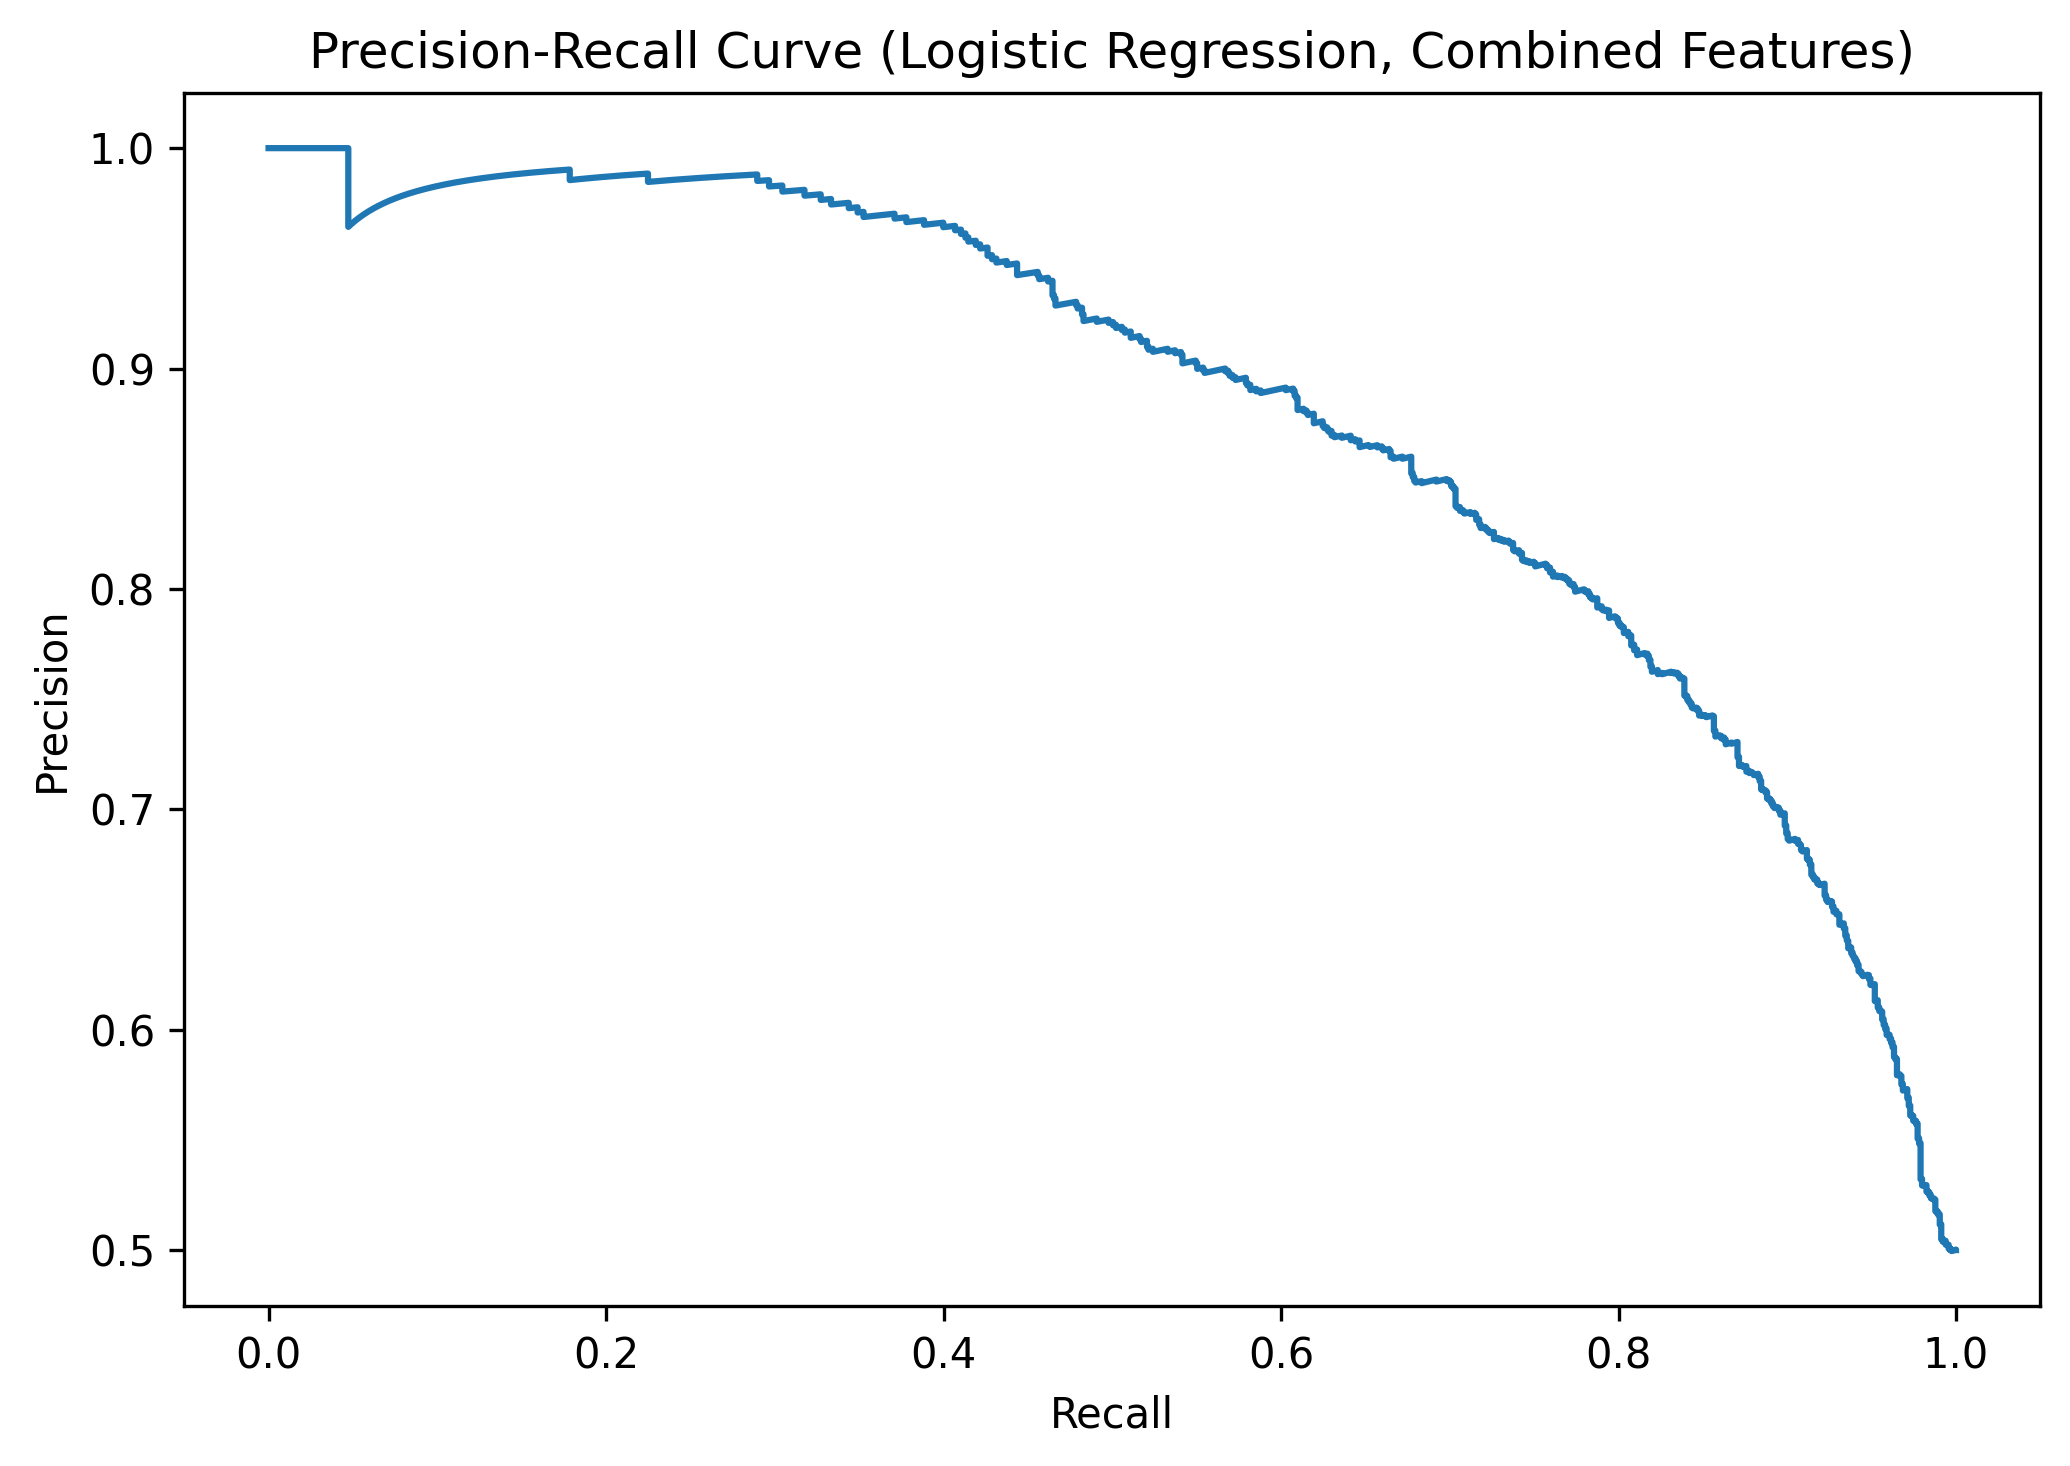
\includegraphics[width=0.48\textwidth]{figures/q2_pr_combined_lr.png}
\caption{Precision-Recall curve for Logistic Regression (combined).}
\label{fig:q2-pr}
\end{figure}

\begin{figure}[H]
\centering
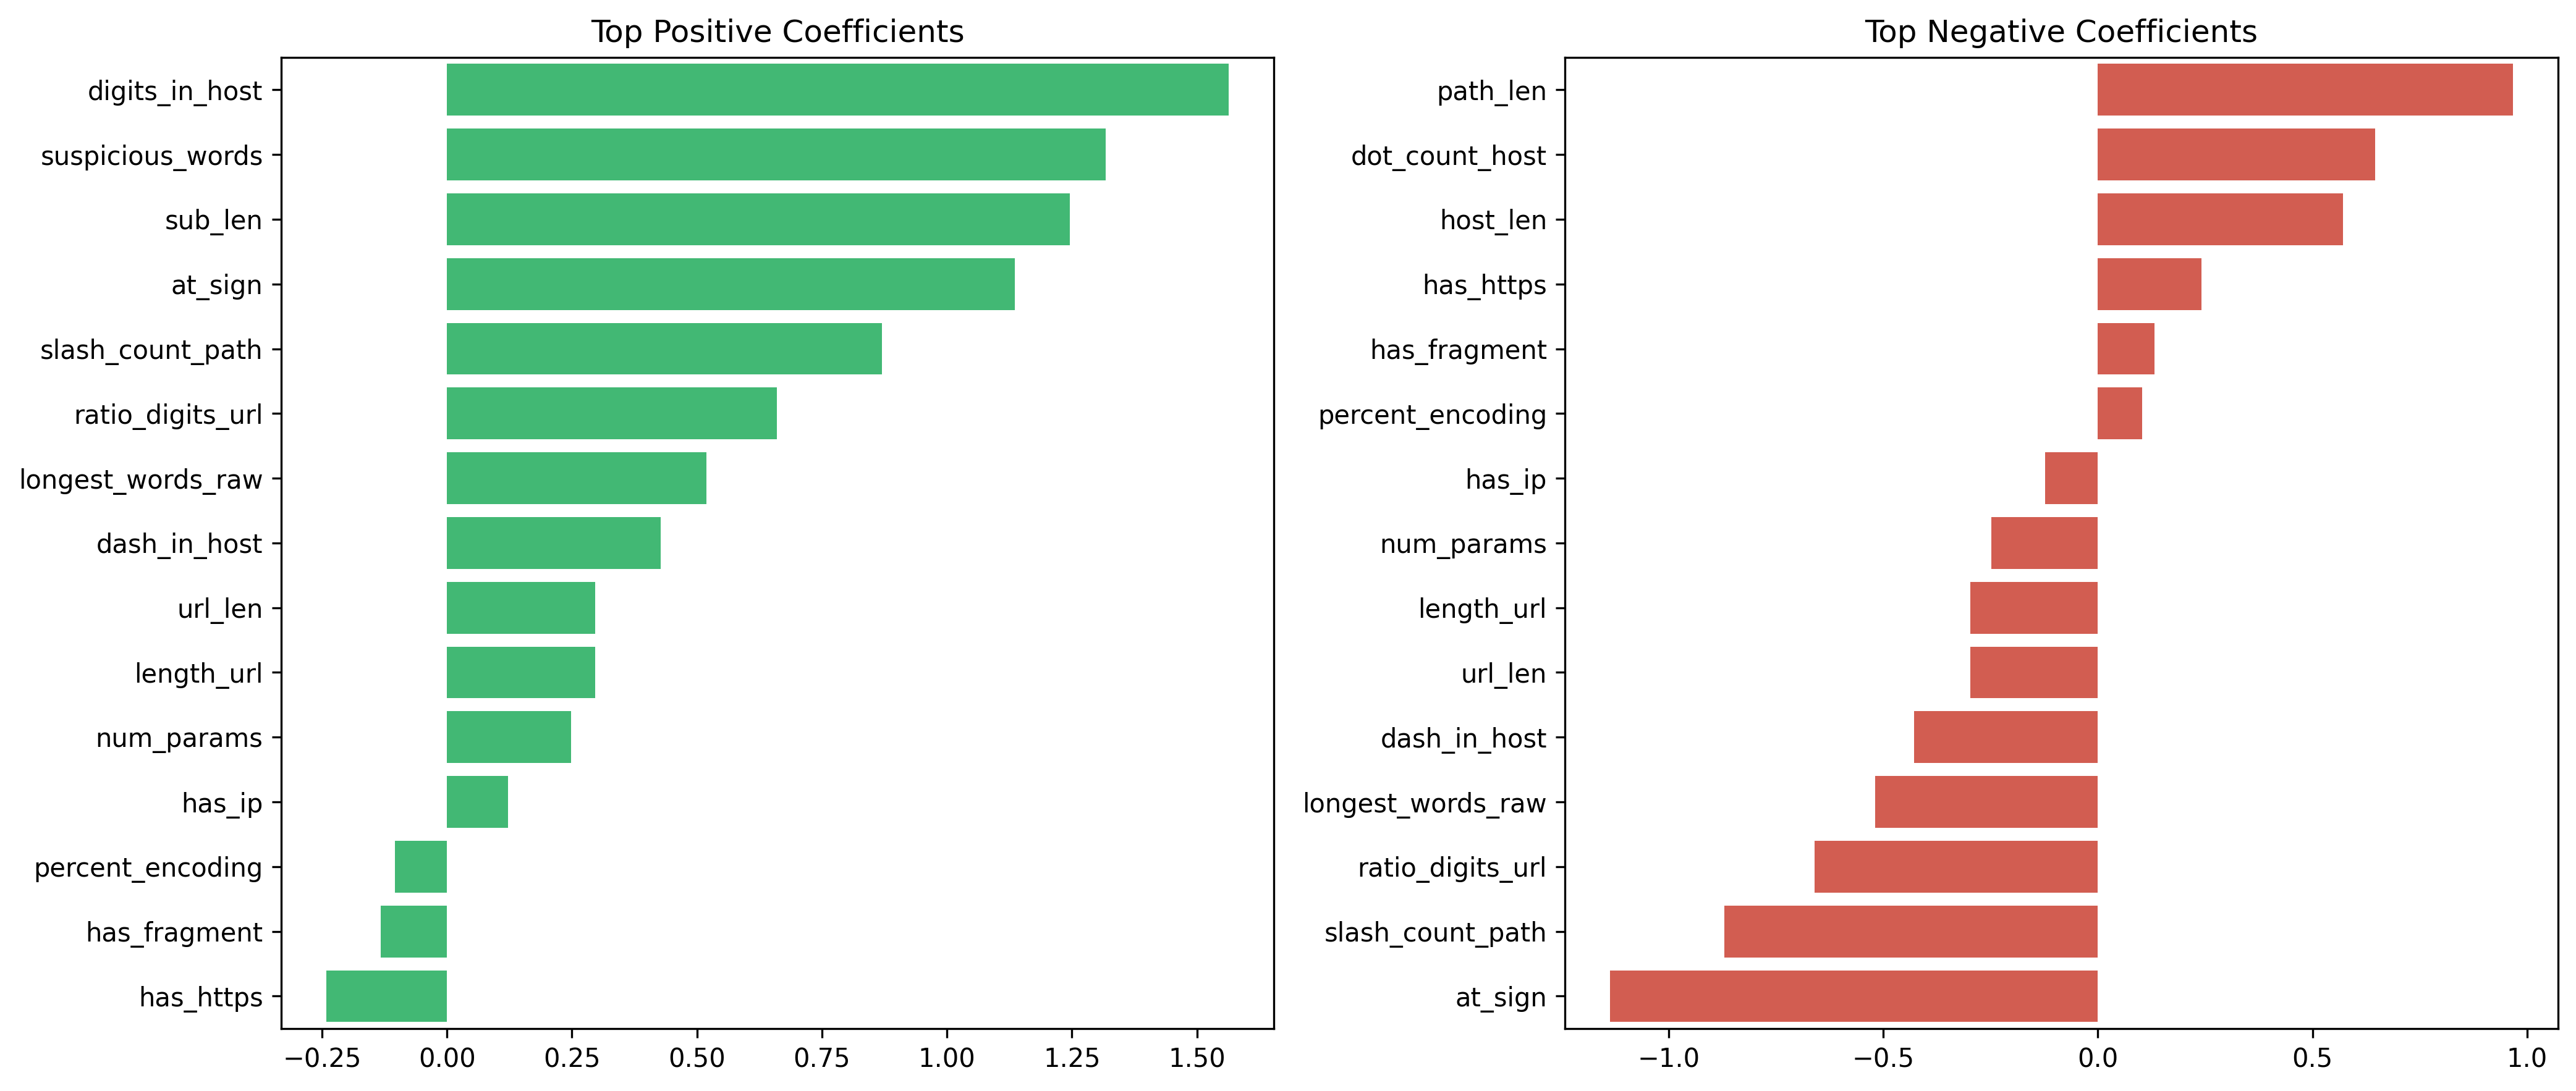
\includegraphics[width=0.48\textwidth]{figures/q2_lr_feature_importance.png}
\caption{Top positive/negative Logistic Regression coefficients.}
\label{fig:q2-coef}
\end{figure}

Figures~\ref{fig:q2-roc} and \ref{fig:q2-pr} indicate stronger ranking consistency for Logistic Regression. The coefficient view in Figure~\ref{fig:q2-coef} also confirms that multiple feature families contribute, validating the combined-feature strategy.

\subsection{Model Tradeoff Interpretation}

Naive Bayes demonstrates a conservative positive prediction tendency in this dataset, reflected by high precision but low recall. Logistic Regression provides a better balance and higher F1-score, which is generally more desirable when both false alarms and misses are costly.

From an operational perspective:
\begin{itemize}
    \item If minimizing false positives is the primary objective, Naive Bayes can be acceptable with threshold tuning.
    \item If balanced detection quality is required, Logistic Regression with combined features is the preferred choice.
\end{itemize}

\section{Discussion, Limitations, and Reproducibility Notes}

\subsection{Cross-Question Synthesis}

Across both questions, a consistent pattern emerges: discriminative linear models (Logistic Regression) provide stronger balanced performance when feature interactions matter. This was evident in sparse lexical email data and became even clearer in heterogeneous URL features.

However, the analysis also confirms that Naive Bayes remains a strong baseline with favorable simplicity-speed tradeoffs. It can produce highly precise alerts in some settings, which may be useful in staged triage pipelines.

\subsection{Engineering Fixes Required for Completion}

Completing this assignment to production-quality required several non-trivial fixes beyond filling placeholder cells:
\begin{enumerate}
    \item \textbf{Deterministic data loading:} all notebook loaders now use fixed project paths under \texttt{datasets/q1} and \texttt{datasets/q2}.
    \item \textbf{Label normalization guards:} explicit mappings for \texttt{spam/ham}, \texttt{Prediction}, and \texttt{phishing/legitimate} avoid silent type drift.
    \item \textbf{Safe stratification logic:} split strategy now handles edge cases cleanly instead of crashing.
    \item \textbf{Dependency handling:} runtime installation cells were replaced by deterministic import guards and environment-level dependency setup.
    \item \textbf{Figure export pipeline:} all report plots are saved with stable filenames for direct LaTeX inclusion.
\end{enumerate}

These changes converted the notebook from a partially interactive artifact to a reproducible experiment pipeline.

\subsection{Threats to Validity}

Despite successful completion, several limitations remain:
\begin{itemize}
    \item \textbf{Single split evaluation:} results are based on one train/test split; cross-validation would reduce variance.
    \item \textbf{Feature scope:} URL-only features exclude external signals such as DNS, WHOIS age, and content rendering behavior.
    \item \textbf{Model complexity:} only linear and Naive Bayes baselines were explored; tree-based ensembles or calibrated boosting could improve detection.
    \item \textbf{Cost-sensitive tuning:} thresholds were not optimized for domain-specific misclassification costs.
\end{itemize}

\subsection{Ablation-Oriented Interpretation}

Feature family ablation in Q2 provides a clear hierarchy:
\begin{enumerate}
    \item Combined features provide the best overall performance.
    \item Creative handcrafted features outperform purely structural or simple statistical signals.
    \item Statistical/content-only features are informative but insufficient alone for robust classification.
\end{enumerate}

This pattern supports the intuition that phishing URLs are best captured through multi-view representation rather than one-dimensional heuristics.

\subsection{Reproducibility Checklist}

The final artifact satisfies the following reproducibility criteria:
\begin{itemize}
    \item One-command notebook execution from project root in the provided virtual environment.
    \item Zero runtime cell errors in a full top-to-bottom run.
    \item Deterministic generation of all expected report figures.
    \item IEEE report compilation from local LaTeX sources without manual post-processing.
\end{itemize}

These properties ensure that another evaluator can re-run the entire pipeline and recover both notebook outputs and PDF report figures.

\section{Conclusion}

This report delivered a complete end-to-end implementation of Assignment 2 with executable code, quantitative evaluation, and publication-style documentation.

In Question 1, from-scratch Logistic Regression and Multinomial Naive Bayes were implemented and compared on email spam detection. Logistic Regression achieved stronger performance on all reported metrics and produced the best overall balance of precision and recall.

In Question 2, URL phishing detection experiments showed that feature engineering quality is the dominant performance driver. Combined structural, statistical, and creative features significantly improved both models, with Logistic Regression again offering the highest balanced effectiveness.

Beyond model metrics, the assignment was completed as a reproducible engineering artifact. Deterministic data paths, robust label mapping, dependency guards, stable split logic, and automatic figure export transformed the notebook into a report-ready experimental workflow.

Future improvements should focus on richer external phishing signals, cross-validated benchmarking, calibration under operational costs, and broader model families. Nevertheless, the current submission satisfies both the academic requirements and practical standards for transparent, rerunnable experimentation.


\bibliographystyle{IEEEtran}
\bibliography{references}

\end{document}
